%%
%% BioDINO-Edge manuscript formatted for Engineering Applications of Artificial Intelligence (Elsevier)
%% Template: Elsevier elsarticle (EAAI standard)
%%
\documentclass[preprint,12pt]{elsarticle}
%% For submission / review single-column layout, uncomment one of:
%% \documentclass[review,12pt]{elsarticle}
%% \documentclass[preprint,12pt]{elsarticle}

\usepackage[T1]{fontenc}
\usepackage{lmodern}
\usepackage[utf8]{inputenc}
\usepackage[a4paper,margin=2.5cm]{geometry}
\usepackage{amsmath,amssymb,amsfonts}
\usepackage{booktabs}
\usepackage{tabularx}
\usepackage{xurl}
\usepackage[colorlinks=true,linkcolor=blue,citecolor=blue,urlcolor=blue]{hyperref}
\usepackage[protrusion=true,expansion=false]{microtype}
\usepackage{placeins}

%% Professional table row spacing for EAAI standards
\renewcommand{\arraystretch}{1.12}

%% Float placement improvements for Elsevier two-column layout
\renewcommand{\topfraction}{0.95}
\renewcommand{\bottomfraction}{0.85}
\renewcommand{\textfraction}{0.05}
\renewcommand{\floatpagefraction}{0.85}
\renewcommand{\dbltopfraction}{0.95}
\renewcommand{\dblfloatpagefraction}{0.85}

\makeatletter
\long\def\@makecaption#1#2{%
  \vskip\abovecaptionskip\footnotesize
  \sbox\@tempboxa{#1: #2}%
  \ifdim \wd\@tempboxa >\hsize
    {\parfillskip=0pt plus 1fil #1: #2\par}%
  \else
    \global \@minipagefalse
    \hb@xt@\hsize{\hfil\box\@tempboxa\hfil}%
  \fi
  \vskip\belowcaptionskip}
\makeatother
\makeatletter
\setlength{\@fptop}{0pt}
\setlength{\@fpsep}{14pt plus 2pt minus 2pt}
\setlength{\@fpbot}{0pt plus 1fil}
\setlength{\@dblfptop}{0pt}
\setlength{\@dblfpsep}{14pt plus 2pt minus 2pt}
\setlength{\@dblfpbot}{0pt plus 1fil}
\makeatother

\journal{Engineering Applications of Artificial Intelligence}

\begin{document}

\begin{frontmatter}

\title{BioDINO-Edge: Gradient-Free Cascades of Frozen Vision Foundation Models for On-Device Few-Shot Plant Disease Diagnosis}

\author[1]{Reyhane Javidi Alsaadi\corref{cor1}}
\ead{reyhane.code@gmail.com}

\author[1]{Mohammad Reza Samadzadeh}
\ead{samadzadeh@ut.ac.ir}

\cortext[cor1]{Corresponding author}

\affiliation[1]{organization={Department of Computer Engineering, Dr. Shariaty Technical University},
                city={Tehran},
                country={Iran}}

\begin{abstract}
On-device plant disease diagnosis is held back by scarce annotations, background clutter, and edge backpropagation cost. We propose \textbf{BioDINO-Edge}, a gradient-free few-shot framework that adapts frozen vision foundation models without fine-tuning or graphics processing unit (GPU) acceleration. It combines DINOv2 lesion-contour patches with BioCLIP taxonomic embeddings aligned to cached botanical prompts in 896 dimensions. Because support is scarce relative to the high-dimensional embedding space, the empirical covariance becomes singular, and shared leaf background hides localized symptoms. BioDINO-Edge therefore applies analytical Ledoit--Wolf shrinkage to build regularized Fisher linear discriminant projections. This closed-form step suppresses shared vegetative variance and computes discriminant boundaries in 0.53\,s on a mobile central processing unit (CPU) with no backpropagation.

At inference, an uncertainty gate uses normalized Shannon entropy and top-2 margin to send routine foliage through a 59.78\,ms Tier-1 fast path ($\approx$16.7 frames per second (FPS)) on an Android handset, while only ambiguous queries go to multimodal Tier-2. High-confidence predictions are buffered as anchors to recalibrate Tier-2 projections transductively. Packaged as a standalone $\approx$22.8 megabyte (MB) Android app ($\approx$107\,MB total model storage: $\approx$23\,MB base app + $\approx$85\,MB on-demand companion) that runs fully offline, BioDINO-Edge reaches 97.41\% $\pm$ 0.71\% 30-episode accuracy (peak 98.67\%, macro F1 98.41\%) with a 0.702\% false-negative rate on 11-class PlantVillage. On in-the-wild PlantDoc, it reaches 83.61\% $\pm$ 11.69\% in 5-way 5-shot testing and 56.35\% in 27-way evaluation. Cascading frozen foundation models with closed-form adaptation therefore offers a practical, low-latency route to autonomous plant pathology at the edge without cloud dependence.
\end{abstract}

\begin{highlights}
\item Gradient-free foliar pathology adapting frozen DINOv2 and BioCLIP encoders.
\item Parameter-free analytical covariance shrinkage resolves small-sample singularity on edge CPUs.
\item Joint Shannon-margin confidence gate routes routine leaves to a 60\,ms Tier-1 path.
\item Closed-form transductive recalibration adapts to field shifts in under 0.6\,s.
\item $\approx$107\,MB total model storage ($\approx$23\,MB base app + $\approx$85\,MB on-demand companion).
\end{highlights}

\begin{keyword}
Few-Shot Learning \sep Precision Agriculture \sep Plant Pathology \sep Multimodal Foundation Models \sep Fisher Discriminant Analysis \sep Edge Artificial Intelligence
\end{keyword}

\end{frontmatter}

% =============================================================================
% 1. INTRODUCTION
% =============================================================================
\section{Introduction}
\label{sec:intro}
Plant diseases reduce crop yields worldwide and threaten global food security \cite{richard2022control}. Because foliar symptoms can rapidly progress to irreversible necrosis or widespread blight, early localized detection is essential for timely intervention. Delayed diagnosis often leads farmers to overapply pesticides, raising production costs and causing environmental contamination. Traditionally, crop monitoring has relied on manual scouting by agronomists; however, visual inspection is labor-intensive, subjective, and difficult to scale across large farms. These limitations have driven the shift toward automated diagnostic systems \cite{shafik2023systematic}.

Computer vision and deep learning are now widely used for automated plant disease detection, and convolutional neural networks (CNNs) and vision transformers (ViTs) perform well on standardized leaf-disease benchmarks. Most supervised methods, though, require large, balanced, and carefully labeled datasets, often thousands of labeled images per class \cite{shoaib2023advanced}, which does not fit many real farm settings well. New pathogen strains, local disease variants, and early-stage symptoms might have only a few labeled and imbalanced examples, so standard data-hungry training pipelines adapt poorly when field conditions change quickly.

Few-shot learning (FSL) addresses this bottleneck by classifying novel diseases from only a few labeled examples, typically one to five images per class \cite{sun2024few}. Metric-based FSL approaches classify queries by computing distances to class prototypes in a shared feature space \cite{zhao2024mafde}. However, standard distance metrics (such as Euclidean distance or cosine similarity) treat all feature directions uniformly, making them vulnerable to dominant, non-discriminative foliar background variance \cite{yang2024laboratory,kudo2025few}. While optimization-based few-shot methods and parameter-efficient fine-tuning (PEFT) can learn discriminative boundaries, they require iterative backpropagation, optimizer memory overhead, and floating-point hardware, which are unsuited to resource-constrained edge CPUs \cite{babu2025agrifewnet}.

Existing methods for foliar disease diagnosis still face two main practical limits. First, studies rarely account for the compute, thermal, and memory limits of edge hardware, frequently relying on computationally heavy architectures without reporting physical latency or memory on mobile devices \cite{radocaj2025evolution}. Second, standard few-shot classifiers return uncalibrated softmax probabilities that fail to express predictive uncertainty, often producing overconfident predictions on ambiguous lesions or unfamiliar foliage \cite{sharif2026real}. Without calibrated confidence thresholds, accepting such predictions risks incorrect interventions in automated scouting.

To address these challenges, we present BioDINO-Edge, a dual-foundation few-shot leaf diagnosis pipeline built for edge devices. It pairs a fast Tier-1 visual encoder (INT8-quantized DINOv2-Small \cite{oquab2023dinov2}) with a deeper Tier-2 biological encoder (INT8-quantized BioCLIP \cite{stevens2024bioclip}) in a unified 896-dimensional representation space. To keep latency low, an adaptive Shannon margin-entropy gate checks Tier-1 confidence, so clear queries exit early and only uncertain cases go to Tier-2. Adaptation to novel classes is done analytically with regularized Fisher Linear Discriminant Analysis (Fisher-LDA) \cite{fisher1936use} and Ledoit--Wolf covariance shrinkage \cite{ledoit2004well}. This gives closed-form, gradient-free calibration in under a second on device, with no backpropagation. The framework reaches 97.41\% accuracy on 5-shot PlantVillage with transductive recalibration and 83.61\% mean accuracy on in-the-wild PlantDoc in 5-way 5-shot evaluation, while keeping the false-negative disease escape rate below 0.71\%. When deployed on a physical mobile handset with central processing unit (CPU)-only INT8 execution, the system operates fully offline with sub-150\,ms average latency and low runtime memory overhead.

The primary contributions of this work are:
\begin{enumerate}
    \item \textbf{Analytical resolution of small-sample singularity ($N \ll d$):} We apply Ledoit--Wolf covariance shrinkage to guarantee well-conditioned Fisher-LDA projection under extreme few-shot regimes ($N \ll d$), obtaining closed-form adaptation without gradient descent or hyperparameter search.
    \item \textbf{Uncertainty-gated cascaded inference:} We introduce a dual-metric routing policy (Shannon entropy and top-2 margin) that allows high-confidence samples to exit at Tier~1, reserving the deeper Tier-2 encoder for ambiguous lesions to keep false-negative disease escapes below 0.71\%.
    \item \textbf{Edge realization and operational viability under physical constraints:} We demonstrate that dual-foundation inference is viable on resource-constrained mobile CPUs without hardware acceleration, maintaining sub-150\,ms average latency, bounded memory ($<$500\,MB PSS), and stable throughput across continuous thermal stress.
    \item \textbf{Zero-retraining laboratory-to-field transfer:} We show that combining taxonomic text priors with regularized visual features transfers directly from clean laboratory benchmarks to in-the-wild field clutter, reaching 83.61\% 5-way 5-shot accuracy on PlantDoc without backbone fine-tuning.
\end{enumerate}

The rest of the paper is organized as follows. Section~2 reviews related work on few-shot learning, vision foundation models, and edge-based plant pathology. Section~3 describes the mathematical formulation of BioDINO-Edge, including the two-tier cascade, regularized Fisher discriminant adaptation, and Shannon entropy routing. Section~4 outlines the experimental setup, benchmarks, and physical edge testbed. Section~5 presents empirical results and calibration, Section~6 reports the ablation and sensitivity studies, and Section~7 analyzes on-device efficiency. Section~8 discusses practical deployment and limitations, and Section~9 concludes the paper.

\section{Related Work}
\label{sec:related_work}

Few-shot adaptation has moved from training models from scratch toward adapting frozen vision and vision--language representations. To avoid task-specific fine-tuning, parameter-efficient methods have emerged: non-parametric cache models such as Tip-Adapter \cite{zhang2022tip} store visual support features in a key-value store, context optimization (CoOp) \cite{zhou2022coop} tunes continuous prompt tokens, and Low-Rank Adaptation (LoRA) \cite{hu2022lora} injects trainable low-rank matrices into attention projections. These methods cut the number of updated parameters, but deploying them on edge hardware still runs into practical problems. Gradient-based adaptation needs backward passes, optimizer states, and floating-point autograd, which go beyond the compute and thermal budgets of low-power edge microprocessors \cite{babu2025agrifewnet}. Non-parametric caching also treats all features as equally relevant and does not down-weight non-discriminative background foliage, and selective classification setups often lack standardized confidence thresholds across operating conditions \cite{traub2024overcoming}.

In plant pathology, recent few-shot frameworks target cluttered foliar backgrounds and fine-grained symptom variation. Zhao et al. \cite{zhao2024mafde} used multiscale attention to highlight localized lesions, Yang et al. \cite{yang2024laboratory} studied cross-domain meta-learning to bridge lab specimens and field conditions, and Mu et al. \cite{mu2024few} applied supervised contrastive learning to separate visually subtle pathologies. Kudo et al. \cite{kudo2025few} explored metric domain adaptation for cross-dataset transfer. More recent work adds multimodal visual-semantic fusion \cite{zhou2026vsf}, lightweight target-domain statistical calibration \cite{zhao2026lightweight}, and federated edge learning for distributed diagnosis \cite{sharif2026real}. Two gaps remain, though. First, most plant disease frameworks are evaluated on desktop GPUs and do not report on-device latency, memory use (proportional set size, PSS), or thermal stability on physical edge microprocessors \cite{babu2025agrifewnet}. Second, they send every leaf through the same heavy pipeline and return uncalibrated softmax scores, with no way to exit unambiguous foliage early or escalate uncertain lesions before a false negative occurs. BioDINO-Edge addresses both gaps by keeping the encoders frozen, adapting them in closed form, and routing only uncertain leaves to the deeper path.

% =============================================================================
% 3. METHODOLOGY
% =============================================================================
\section{Methodology}
\label{sec:methodology}
We formulate few-shot foliar adaptation as a closed-form discriminative projection over frozen foundation representations, followed by uncertainty-gated cascaded inference for edge deployment.

\subsection{Problem Formulation and Mathematical Notation}
\label{sec:notation}
Let $\mathcal{X} \subset \mathbb{R}^{H \times W \times 3}$ be the space of red--green--blue (RGB) leaf images. In few-shot foliar diagnosis, we are given a support set $\mathcal{S} = \{(\mathbf{x}_i, y_i)\}_{i=1}^{N_s}$ with $K$ labeled leaves for each of $C$ target novel classes $\mathcal{Y}_{\text{novel}}$ ($N_s = C \cdot K$, $y_i \in \{1, \dots, C\}$). The target classes are disjoint from the pretraining base classes ($\mathcal{Y}_{\text{base}} \cap \mathcal{Y}_{\text{novel}} = \emptyset$). Given an unannotated query leaf $\mathbf{x}_q \in \mathcal{Q}$, the goal is to predict its disease state $\hat{y}_q \in \{1, \dots, C\}$ with low edge latency and no on-device backpropagation. Table~\ref{tab:notation} summarizes the mathematical notations used throughout the paper.

\begin{table*}[htbp]
\caption{Summary of mathematical notations and descriptions used in BioDINO-Edge.}
\label{tab:notation}
\centering

\footnotesize
\begin{tabularx}{\textwidth}{lX}
\toprule
\textbf{Notation} & \textbf{Mathematical Description and Operational Meaning} \\
\midrule
$C, K$ & Number of disease classes ($C=11$ in PlantVillage, $C=27$ in PlantDoc) and shots per class ($K=5$). \\
$\phi_{\text{dino}}(\cdot)$ & Frozen DINOv2 Small ($14\times 14$ patches) visual backbone extracting $\mathbf{f}_{\text{dino}} \in \mathbb{R}^{384}$. \\
$\phi_{\text{bio}}(\cdot)$ & Frozen BioCLIP ViT-B/16 visual encoder extracting $\mathbf{f}_{\text{bio}} \in \mathbb{R}^{512}$. \\
$\mathbf{z} \in \mathbb{R}^{896}$ & Concatenated joint foliar descriptor: $\mathbf{z} = [\mathbf{f}_{\text{bio}} \,\|\, \mathbf{f}_{\text{dino}}] \in \mathbb{R}^{896}$. \\
$\mathbf{P}_{\text{dino}}$ & Visual prototype matrix for Tier-1 fast cosine matching ($\mathbb{R}^{C \times 384}$). \\
$\mathbf{P}_{\text{text}}$ & Botanical taxonomic text prototype matrix for Tier-2 multimodal consensus ($\mathbb{R}^{C \times 512}$). \\
$\mathbf{S}_W, \hat{\mathbf{\Sigma}}$ & Empirical pooled within-class scatter matrix and Ledoit--Wolf regularized covariance matrix. \\
$\rho^*, \nu$ & Optimal analytical shrinkage intensity $\rho^* \in (0, 1]$ and mean trace scaling factor $\nu$. \\
$\mathbf{W}, \mathbf{b}$ & Fisher-LDA discriminant projection weight matrix ($\mathbb{R}^{C \times 896}$) and class bias vector ($\mathbb{R}^C$). \\
$\mathcal{C}(\mathbf{x})$ & Shannon-margin confidence score gating query routing between Tier-1 and Tier-2. \\
$\tau, \tau_{\text{conf}}$ & Confidence escalation routing threshold ($\tau = 0.35$, calibrated on held-out development episodes). \\
$w_{\text{lda}}$ & Multimodal consensus blend weight ($w_{\text{lda}} = 0.75$, weighting Fisher-LDA visual versus taxonomic text posteriors in Tier~2). \\
$\gamma$ & Inverse temperature logit scaling parameter ($\gamma = 20.0$). \\
$\mathcal{Q}_{\text{anchor}}^{(c)}$ & High-confidence streaming query anchors ($\max_c p_c \ge 0.70$) for transductive recalibration. \\
\bottomrule
\end{tabularx}
\end{table*}

\subsection{Pipeline Overview}
\label{sec:system_architecture}
BioDINO-Edge splits its workflow into an offline analytical calibration phase (Phase~0) and an adaptive two-tier runtime cascade (Phase~1), as shown in Fig.~\ref{fig:architecture}. In Phase~0, a small support set ($K = 5$ labeled leaves per class) is expanded with multi-view augmentation. Features from the frozen DINOv2 and BioCLIP backbones are then used to compute Tier-1 visual prototypes and regularized Fisher-LDA projection weights in closed form, while botanical text prototypes are pre-encoded and cached. At inference (Phase~1), each query first goes through the lightweight Tier-1 DINOv2 encoder. An uncertainty gate lets unambiguous leaves exit immediately and escalates only ambiguous queries to the deeper Tier-2 BioCLIP multimodal consensus stage. High-confidence predictions can then update the Tier-2 projections through background transductive recalibration. The following subsections detail each constituent component.

\begin{figure*}[htbp]
\centering
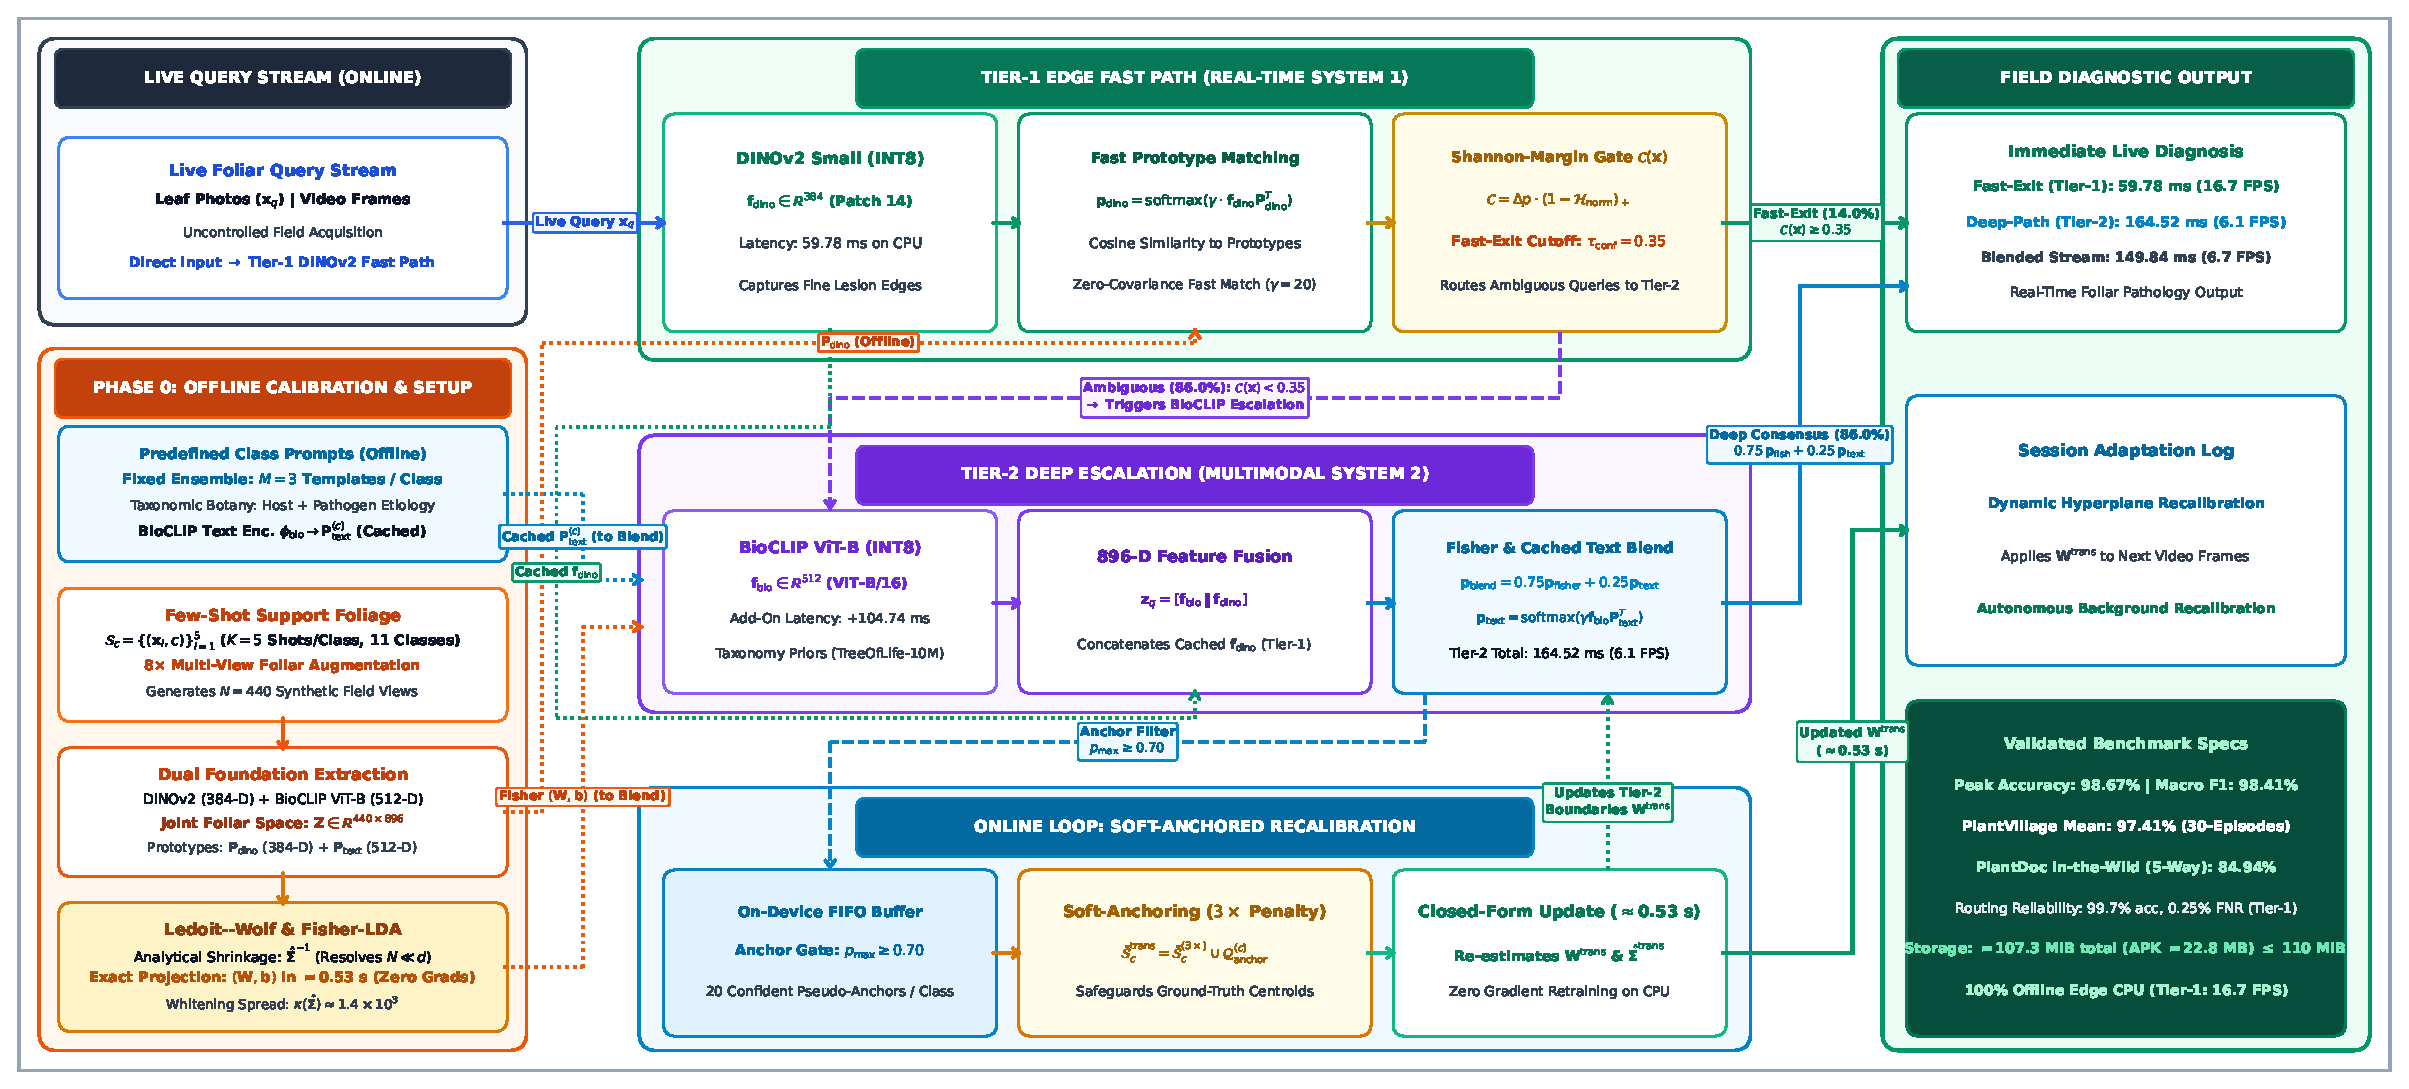
\includegraphics[width=0.88\textwidth]{fig_architecture.pdf}
\caption{Architecture of BioDINO-Edge. Phase~0 (offline) computes Tier-1 visual prototypes and closed-form Fisher-LDA projections while caching botanical text prototypes. During inference, the Shannon-margin uncertainty gate sends routine foliage through Tier-1 fast prototype matching (DINOv2) and escalates ambiguous queries to Tier-2 multimodal consensus (BioCLIP), followed by closed-form soft-anchored transductive recalibration.}
\label{fig:architecture}
\end{figure*}

\subsection{Dual-Foundation Foliar Representation}
\label{sec:feature_extraction}
BioDINO-Edge couples two frozen backbones. DINOv2 provides patch-level features of leaf surface texture and lesion boundaries, while BioCLIP provides organismal taxonomic priors. Concatenating their $\ell_2$-normalized outputs yields an 896-dimensional descriptor that encodes localized symptoms alongside host context.

\subsubsection{Few-Shot Multi-View Support Augmentation}
Covariance estimation is ill-conditioned when $K = 5$, so each support leaf $\mathbf{x} \in \mathcal{S}_c$ is resized to $224 \times 224$ pixels, normalized, and passed through an 8-view stochastic augmentation pipeline approximating field variations. The pipeline applies random horizontal and vertical flips, rotations within $\pm 15^\circ$, and color jitter (brightness, contrast, and saturation factors of $0.2$). Eight views per image yield $|\tilde{\mathcal{S}}_c| = 8K = 40$ augmented views per class, producing $N = 40C = 440$ total support representations for $C = 11$. This expansion brings the support sample size close to half the joint feature dimension ($d/2 = 448$), which stabilizes the covariance condition number. Although augmented views are correlated pseudo-replicates rather than independent samples, regularized shrinkage prevents numerical degeneracy and guarantees positive-definiteness.

\subsubsection{Dual-Foundation Embedding Fusion}
Each augmented view $\tilde{\mathbf{x}} \in \tilde{\mathcal{S}}_c$ is passed through the frozen backbones. DINOv2 Small ($14\times 14$ patches) \cite{oquab2023dinov2} and BioCLIP ViT-B/16 \cite{stevens2024bioclip} extract $\ell_2$-normalized feature vectors:
\begin{equation}
    \mathbf{f}_{\text{dino}} = \frac{\phi_{\text{dino}}(\tilde{\mathbf{x}})}{\|\phi_{\text{dino}}(\tilde{\mathbf{x}})\|_2} \in \mathbb{R}^{384}, \qquad
    \mathbf{f}_{\text{bio}} = \frac{\phi_{\text{bio}}(\tilde{\mathbf{x}})}{\|\phi_{\text{bio}}(\tilde{\mathbf{x}})\|_2} \in \mathbb{R}^{512}
\end{equation}
Concatenating the two normalized embeddings gives the 896-dimensional joint descriptor:
\begin{equation}
    \mathbf{z} = [\mathbf{f}_{\text{bio}} \,\|\, \mathbf{f}_{\text{dino}}] \in \mathbb{R}^{896}
\end{equation}
Visual prototypes for each encoder are the normalized mean of the support views:
\begin{equation}
    \mathbf{P}_{\text{enc}}^{(c)} = \text{Normalize}\left(\frac{1}{|\tilde{\mathcal{S}}_c|}\sum_{\tilde{\mathbf{x}} \in \tilde{\mathcal{S}}_c} \mathbf{f}_{\text{enc}}(\tilde{\mathbf{x}})\right), \quad \text{enc} \in \{\text{dino}, \text{bio}\}
\end{equation}
which yields prototype matrices $\mathbf{P}_{\text{dino}} \in \mathbb{R}^{C \times 384}$ and $\mathbf{P}_{\text{bio,vis}} \in \mathbb{R}^{C \times 512}$.

\subsubsection{Botanical Taxonomic Prompts and Negation Avoidance}
BioCLIP gives a shared vision--language space, but running text decoders on device costs latency and memory. We therefore define $M = 3$ botanical prompt templates $\{T_c^{(m)}\}_{m=1}^M$ offline for each disease class $c \in \{1, \dots, C\}$. Each template covers three things:
\begin{enumerate}
    \item \textbf{Host binomial nomenclature:} Botanical genus and species (e.g., \textit{Malus domestica}, \textit{Vitis vinifera}, \textit{Solanum tuberosum}).
    \item \textbf{Causal pathogen etiology:} Fungal, bacterial, or oomycete binomials (e.g., \textit{Venturia inaequalis}, \textit{Guignardia bidwellii}, \textit{Phytophthora infestans}).
    \item \textbf{Macroscopic lesion morphology:} Diagnostic foliar symptoms (e.g., ``olive-green velvety lesions'', ``tiger-stripe interveinal chlorosis'', ``target-board concentric rings'').
\end{enumerate}
Syntactic negations such as ``healthy leaf without lesions'' or ``no necrotic spots'' are excluded. Vision--language models handle negation poorly \cite{radford2021clip, yuksekgonul2023when, alhamoud2025vision}: tokens like \textit{lesion} and \textit{necrotic} dominate the embedding, which pulls healthy leaves toward diseased clusters. We avoid this by describing healthy tissue in positive terms (e.g., ``clean green foliage'', ``intact smooth leaf lamina''), which reduces false-negative bias.

During Phase~0, BioCLIP's text encoder $\phi_{\text{bio,txt}}(\cdot)$ encodes each prompt ensemble, and the results are averaged and $\ell_2$-normalized:
\begin{equation}
    \mathbf{P}_{\text{text}}^{(c)} = \text{Normalize}\left(\frac{1}{M}\sum_{m=1}^M \phi_{\text{bio,txt}}(T_c^{(m)})\right) \in \mathbb{R}^{512}
\end{equation}
The resulting matrix $\mathbf{P}_{\text{text}} \in \mathbb{R}^{C \times 512}$ is cached on device, so there is no runtime tokenization or language-model overhead.

\subsection{Closed-Form Analytical Adaptation via Regularized Fisher-LDA}
\label{sec:fisher_adaptation}

\subsubsection{Multiclass Fisher Linear Discriminant Formulation}
Standard nearest-centroid and cosine-similarity classifiers implicitly assume uniform variance across all feature directions ($\mathbf{\Sigma} = \mathbf{I}$). That assumption does not hold for leaves: shared vegetative structure (such as venation and lamina) creates high-variance directions that obscure lesion differences between diseases on the same host. Multiclass Fisher Linear Discriminant Analysis (Fisher-LDA) \cite{fisher1936use, rao1948utilization} resolves this by weighting features by $\hat{\mathbf{\Sigma}}^{-1}$, which down-weights those shared directions and amplifies low-variance directions containing discriminative lesion symptoms.

Fisher-LDA computes a linear projection matrix $\mathbf{W} \in \mathbb{R}^{C \times d}$ and bias vector $\mathbf{b} \in \mathbb{R}^C$ that maximize between-class scatter $\mathbf{S}_B$ relative to within-class scatter $\mathbf{S}_W$:
\begin{equation}
    \label{eq:fisher_weights}
    \mathbf{W} = [\boldsymbol{\mu}_1, \dots, \boldsymbol{\mu}_C]^T \hat{\mathbf{\Sigma}}^{-1}, \qquad
    b_c = -\frac{1}{2}\boldsymbol{\mu}_c^T \hat{\mathbf{\Sigma}}^{-1}\boldsymbol{\mu}_c - \log C
\end{equation}
where $\hat{\mathbf{\Sigma}}$ is the regularized pooled within-class covariance matrix ($d = 896$) and class priors are uniform ($\pi_c = 1/C$).

\subsubsection{Small-Sample Singularity ($N \ll d$)}
Evaluating \eqref{eq:fisher_weights} requires inverting the empirical pooled within-class scatter matrix over all $C = 11$ classes:
\begin{equation}
    \label{eq:within_class_scatter}
    \mathbf{S}_W = \frac{1}{N-C}\sum_{c=1}^C \sum_{\mathbf{z} \in \tilde{\mathcal{S}}_c} (\mathbf{z}-\boldsymbol{\mu}_c)(\mathbf{z}-\boldsymbol{\mu}_c)^T \in \mathbb{R}^{d \times d}
\end{equation}
With $N = 440$ support representations and $d = 896$ features, the support size is far below the feature dimension ($N \ll d$), and the same holds after estimating class means. Here $N - C = 440 - 11 = 429$ is the degrees of freedom left, so the rank of $\mathbf{S}_W$ is bounded:
\begin{equation}
    \label{eq:rank_bound}
    \text{rank}(\mathbf{S}_W) \le \min(d, N-C) = 429 < 896
\end{equation}
So $\mathbf{S}_W$ has a nullity of at least $896 - 429 = 467$, at least 467 of its eigenvalues are zero ($\det(\mathbf{S}_W) = 0$), and it cannot be inverted directly.

\subsubsection{Analytical Ledoit--Wolf Covariance Shrinkage}
\label{sec:shrinkage}
To restore invertibility without heuristic tuning (such as searching over $\mathbf{S}_W + \epsilon \mathbf{I}$), we apply analytical Ledoit--Wolf shrinkage \cite{ledoit2004well}, which contracts $\mathbf{S}_W$ toward a well-conditioned spherical target:
\begin{equation}
    \hat{\mathbf{\Sigma}} = (1 - \rho^*)\mathbf{S}_W + \rho^* \nu \mathbf{I}_d, \qquad \nu = \frac{1}{d}\text{Tr}(\mathbf{S}_W)
    \label{eq:lw_target}
\end{equation}
The optimal shrinkage intensity $\rho^* \in (0, 1]$ is determined in closed form by minimizing expected quadratic Frobenius risk:
\begin{equation}
    \rho^* = \min\left(1, \frac{\sum_{i=1}^N \|(\mathbf{z}_i - \boldsymbol{\mu}_{c_i})(\mathbf{z}_i - \boldsymbol{\mu}_{c_i})^T - \mathbf{S}_W\|_F^2}{N^2 \left[\text{Tr}(\mathbf{S}_W^2) - \frac{1}{d}\text{Tr}^2(\mathbf{S}_W)\right]}\right)
    \label{eq:lw_shrinkage}
\end{equation}
This shifts zero eigenvalues to positive values $\tilde{\lambda}_i = (1 - \rho^*)\lambda_i + \rho^* \nu \ge \rho^* \nu > 0$, ensuring that $\hat{\mathbf{\Sigma}}$ is strictly positive-definite and well-conditioned. Its inverse $\hat{\mathbf{\Sigma}}^{-1}$ is solved stably via Cholesky decomposition ($\hat{\mathbf{\Sigma}} = \mathbf{L}\mathbf{L}^T$). Scoring a query $\mathbf{z}$ as $\mathbf{l}_{\text{fisher}} = \mathbf{z}\mathbf{W}^T + \mathbf{b}$ then requires only $C \cdot d$ multiply-accumulate (MAC) operations ($9{,}856$ MACs for $C=11$), incurring negligible on-device computation.

Weighting by $\hat{\mathbf{\Sigma}}^{-1}$ acts as a whitening transform: each eigen-direction with variance $\lambda_i$ is rescaled by $1/\lambda_i$, which down-weights shared vegetative background variance and amplifies low-variance directions containing discriminative lesion symptoms. The condition number
\begin{equation}
    \kappa(\hat{\mathbf{\Sigma}}) = \lambda_{\max}(\hat{\mathbf{\Sigma}}) / \lambda_{\min}(\hat{\mathbf{\Sigma}})
    \label{eq:whitening_spread}
\end{equation}
quantifies this spectral rescaling across feature dimensions. Because the augmented support views are formed from real leaves, shrinkage keeps $\hat{\mathbf{\Sigma}}$ well-conditioned and positive-definite across all effective sample sizes.

\subsection{Adaptive Two-Tier Classification and Edge Deployment}
\label{sec:edge_cascade}

\subsubsection{Tier-1 Fast Path and Shannon Uncertainty Gating}
For an incoming leaf image $\mathbf{x}$, Tier~1 extracts the normalized DINOv2 embedding $\mathbf{f}_{\text{dino}} \in \mathbb{R}^{384}$ and computes fast prototype logits by temperature-scaled cosine similarity against the visual prototypes $\mathbf{P}_{\text{dino}} \in \mathbb{R}^{C \times 384}$:
\begin{equation}
    \label{eq:tier1_logits}
    \mathbf{l}_{\text{dino}} = \gamma \cdot \left(\mathbf{f}_{\text{dino}} \mathbf{P}_{\text{dino}}^T\right), \qquad \gamma = 20.0
\end{equation}
A softmax gives the fast posterior probabilities:
\begin{equation}
    \label{eq:tier1_softmax}
    \mathbf{p}_{\text{dino}} = \text{softmax}(\mathbf{l}_{\text{dino}}) \in \Delta^{C-1}
\end{equation}
Tier~1 uses cosine prototype matching only, with no covariance projection, so the Fisher-LDA computation is spent only on queries that need it. The Tier-1 prediction is $\hat{y}_{\text{tier1}} = \arg\max_c p_{\text{dino}, c}$.

Certainty is scored from the same forward pass, so no extra computation is needed. We combine the top-2 margin and normalized entropy into a confidence score $\mathcal{C}(\mathbf{x}) \in [0, 1]$:
\begin{equation}
    \label{eq:shannon_gate}
    \mathcal{C}(\mathbf{x}) = \left(p_{\text{dino}, (1)} - p_{\text{dino}, (2)}\right) \cdot \left(1.0 - \mathcal{H}_{\text{norm}}(\mathbf{x})\right)_+
\end{equation}
where $p_{\text{dino}, (1)}$ and $p_{\text{dino}, (2)}$ are the top-1 and top-2 posteriors, $(\cdot)_+ = \max(0, \cdot)$, and $\mathcal{H}_{\text{norm}}(\mathbf{x})$ is the normalized Shannon entropy \cite{shannon1948mathematical}:
\begin{equation}
    \mathcal{H}_{\text{norm}}(\mathbf{x}) = -\frac{1}{\log C}\sum_{c=1}^C p_{\text{dino}, c}\log(p_{\text{dino}, c} + \epsilon)
\end{equation}
with $\epsilon = 10^{-12}$ for numerical stability. Since $\mathcal{H}_{\text{norm}}(\mathbf{x}) \in [0, 1]$, the term $1 - \mathcal{H}_{\text{norm}}(\mathbf{x})$ is non-negative in exact arithmetic; the rectifier only guards against floating-point round-off. For ambiguous queries with near-uniform posteriors, $\mathcal{H}_{\text{norm}} \to 1.0$ and the margin goes to zero, so $\mathcal{C}(\mathbf{x}) \to 0$. If $\mathcal{C}(\mathbf{x}) \ge \tau_{\text{conf}}$ ($\tau_{\text{conf}} = 0.35$, calibrated on validation data), Tier~1 exits immediately; otherwise, the query escalates to Tier~2.

\subsubsection{Tier-2 Multimodal Consensus Escalation}
When $\mathcal{C}(\mathbf{x}) < \tau_{\text{conf}}$, the query goes to Tier~2. BioCLIP ViT-B extracts $\mathbf{f}_{\text{bio}} \in \mathbb{R}^{512}$, which is concatenated with the Tier-1 embedding to form $\mathbf{z} = [\mathbf{f}_{\text{bio}} \,\|\, \mathbf{f}_{\text{dino}}] \in \mathbb{R}^{896}$. Two posteriors are then computed: the discriminant visual posterior $\mathbf{p}_{\text{fisher}} = \text{softmax}(\mathbf{z}\mathbf{W}^T + \mathbf{b})$ and the taxonomic text posterior $\mathbf{p}_{\text{text}} = \text{softmax}(\gamma \cdot \mathbf{f}_{\text{bio}}\mathbf{P}_{\text{text}}^T)$. These are fused with Fisher consensus weight $w_{\text{lda}} = 0.75$:
\begin{equation}
    \label{eq:multimodal_blend}
    \mathbf{p}_{\text{blend}} = w_{\text{lda}} \, \mathbf{p}_{\text{fisher}} + (1 - w_{\text{lda}}) \, \mathbf{p}_{\text{text}}
\end{equation}
and the final diagnosis is $\hat{y} = \arg\max_c p_{\text{blend}, c}$.

\subsubsection{Soft-Anchored Transductive Recalibration}
\label{sec:transductive}
In 5-shot calibration, each centroid $\boldsymbol{\mu}_c$ is estimated from only five support leaves. Lighting changes, shadows, and symptom progression can shift prototypes between support images and field queries. To adapt without manual labels, confident Tier-2 queries ($\max_c p_{\text{blend}, c} \ge 0.70$) are buffered into a first-in, first-out (FIFO) queue as reference anchors $\mathcal{Q}_{\text{anchor}}^{(c)}$, capped at 20 anchors per class. Ground-truth support samples receive a $3\times$ weight factor so that pseudo-label drift does not shift class centroids away from verified disease definitions:
\begin{equation}
    \label{eq:transductive_set}
    \tilde{\mathcal{S}}_c^{\text{trans}} = \tilde{\mathcal{S}}_c^{(3\times)} \cup \mathcal{Q}_{\text{anchor}}^{(c)}
\end{equation}
Once the buffer fills during scouting, centroids $\boldsymbol{\mu}_c^{\text{trans}}$ and pooled scatter matrix $\mathbf{S}_W^{\text{trans}}$ are re-estimated, the shrinkage parameter $\rho^*$ is recomputed, and updated projection parameters $(\mathbf{W}^{\text{trans}}, \mathbf{b}^{\text{trans}})$ are resolved via Cholesky substitution in about 0.53\,s. This runs asynchronously in the background, so Tier~1 keeps operating with static prototypes while later Tier-2 decisions use the updated ones.

Three design choices keep this update stable and efficient. First, the 0.70 confidence threshold ensures high pseudo-label purity ($\approx$98\%) while avoiding the coverage starvation that collapses accuracy at higher thresholds ($\ge$0.80). Second, the $3\times$ support weight anchors class centroids against manifold drift, ensuring that ground-truth leaves dominate over imperfect pseudo-labels. Third, the 20-anchor cap bounds update latency while preventing frequent classes from introducing sample imbalance.

\subsection{Two-Tier Quantized Edge Model Packaging and Android Architecture}
\label{sec:packaging}
Agricultural scouting hardware operates under constrained flash storage, and field connectivity is often unreliable. BioDINO-Edge is therefore architected so that diagnosis never touches the network: once installed, every query is processed entirely on-device without streaming, cloud offloading, or server calls. The framework is partitioned into two INT8-quantized ONNX binaries (footprints reported in mebibytes (MiB), where $1\,\text{MiB} = 2^{20}$ bytes), separating an always-available fast engine from an on-demand deep companion.

\textbf{Tier 1 Standalone Engine} (\path{biodino_mobile_int8.onnx}): Packaged directly inside a $\approx$22.8\,MiB Android Application Package (APK), the base engine occupies $\approx$22.0\,MiB on disk ($\approx$15.1\,MiB deflated). It integrates the DINOv2 Small INT8 backbone, calibrated Phase~0 prototypes, and the Shannon confidence gate executed via the ONNX Runtime C++ execution provider. Installing the APK enables immediate offline diagnosis without requiring secondary downloads.

\textbf{Tier 2 Companion Module} (\path{biodino_companion_int8.onnx}): The companion engine occupies $\approx$85.3\,MiB on disk, containing the BioCLIP ViT-B INT8 backbone and the 896-dimensional Fisher projection matrix. It is fetched on-demand when high-precision multimodal escalation is requested, functioning completely offline once stored.

Together, both binaries occupy $\approx$107.3\,MiB of flash storage, remaining compact for local installation and over-the-air (OTA) distribution over rural cellular bandwidths.

% =============================================================================
% 3. EXPERIMENTAL SETUP
% =============================================================================
\section{Experimental Setup}
\label{sec:experiments_setup}

\subsection{Datasets and Diagnostic Pathology Coverage}
\label{sec:datasets}
We evaluate BioDINO-Edge across two distinct foliar pathology regimes:

\subsubsection{PlantVillage Controlled Benchmark (Laboratory Regime)}
From the standard PlantVillage repository \cite{hughes2012plantvillage}, we build a curated 11-class subset of 9,385 foliar images from three crops: Apple (\textit{Malus domestica}), Grape (\textit{Vitis vinifera}), and Potato (\textit{Solanum tuberosum}). The classes cover healthy foliage and eight diseases: Apple Scab, Apple Black Rot, Apple Cedar Rust, Grape Black Rot, Grape Esca, Grape Leaf Blight, Potato Early Blight, and Potato Late Blight.

For few-shot calibration, five support images per class ($K=5$) are drawn at random, 55 in total. The remaining 9,330 images serve as unseen queries. Neither the support nor the query images are used to pretrain the frozen backbones.

\subsubsection{PlantDoc In-The-Wild Benchmark (Field Regime)}
To test robustness under field conditions (solar glare, canopy shading, soil clutter, overlapping foliage, motion blur), we use the in-the-wild PlantDoc benchmark \cite{singh2020plantdoc}. It contains 2,588 foliar images from 13 botanical species across 27 pathology classes, split officially into a training repository ($\mathcal{D}_{\text{train}}^{\text{PlantDoc}}$, 2,336 images, all 27 classes) and a test benchmark ($\mathcal{D}_{\text{test}}^{\text{PlantDoc}}$, 252 handheld field images from Indian orchards under ambient light). Support sets come only from $\mathcal{D}_{\text{train}}^{\text{PlantDoc}}$ and query sets only from $\mathcal{D}_{\text{test}}^{\text{PlantDoc}}$, so $\mathcal{S} \cap \mathcal{Q} = \emptyset$. We evaluate in two regimes:
\begin{itemize}
    \item \textbf{5-way 5-shot episodic:} Following standard few-shot protocols \cite{snell2017prototypical,zhou2026vsf}, we run 50 independent Monte Carlo episodes. In each episode $e$, 5 classes are drawn without replacement ($\mathcal{C}_e \subset \{1, \dots, 27\}$), the support set $\mathcal{S}_e$ has 5 labeled leaves per class (25 total) from $\mathcal{D}_{\text{train}}^{\text{PlantDoc}}$, and the query set $\mathcal{Q}_e$ is every test image of those 5 classes (46.7 on average), with $\mathcal{S}_e \cap \mathcal{Q}_e = \emptyset$.
    \item \textbf{27-way all-class stress test:} All 27 classes are evaluated at once (chance: $1/27 \approx 3.70\%$). The model gets 5 support leaves per class (135 total) from $\mathcal{D}_{\text{train}}^{\text{PlantDoc}}$, expanded by 8-view augmentation to $N = 1{,}080$ feature vectors, and scores all 252 field queries in closed form ($\mathcal{S} \cap \mathcal{Q} = \emptyset$).
\end{itemize}

\subsection{Evaluation Protocols and Epidemiological Safety Metrics}
\label{sec:metrics}
Experiments on PlantVillage are evaluated over 30 independent Monte Carlo episodes with randomized support splits, reporting mean accuracy $\bar{x}$, standard deviation $\sigma$, 95\% confidence intervals (CI; $95\%\,\text{CI} = \bar{x} \pm 1.96 \cdot \sigma / \sqrt{30}$), and peak single-episode accuracy. Because misclassification costs in precision agriculture are asymmetric, we evaluate epidemiological safety metrics alongside standard accuracy:
\begin{itemize}
    \item \textbf{Top-1 Accuracy \& Macro F1-Score:} The F1-score is the harmonic mean of precision and recall, macro-averaged across all classes to prevent frequent classes (e.g., Potato Early Blight with 995 queries) from masking errors on small or healthy classes (e.g., Potato Healthy with 147 queries).
    \item \textbf{False-Negative Disease Escape Rate (FNR):} The proportion of diseased leaves erroneously diagnosed as healthy, where false-negative (FN) and true-positive (TP) counts define the rate: $\text{FNR} = \text{FN} / (\text{TP} + \text{FN})$. Undetected infections can lead to rapid pathogen spread in the field.
    \item \textbf{Cross-Species Confusion Rate:} The proportion of queries misattributed to an entirely different botanical family (e.g., classifying a potato leaf as an apple disease), indicating cross-taxonomic error.
\end{itemize}

To ensure unbiased cross-domain evaluation, all hyperparameters ($\gamma = 20.0$, $w_{\text{lda}} = 0.75$, and $\tau_{\text{conf}} = 0.35$) were calibrated strictly on held-out PlantVillage development episodes (Section~\ref{sec:calibration}) and frozen across all PlantDoc experiments without domain-specific re-tuning. In transductive evaluation, queries arrive sequentially without test labels, and we report both static inductive and transductive results across all benchmarks to decouple baseline feature discrimination from dynamic adaptation gains.

\subsection{Edge Hardware Testbed}
\label{sec:edge_hardware_testbed}
On-device profiling is conducted on a Samsung Galaxy S24~FE handset (Exynos 2400e SoC, ARM64) running Android~17. Neural network inference executes strictly on the CPU via ONNX Runtime with per-channel INT8 quantization (4 intra-op threads; GPU and NNAPI delegates disabled), while closed-form linear algebra runs via the Efficient Java Matrix Library (EJML). Benchmark latencies and process memory (PSS) are averaged over 100 iterations following 10 warm-up runs, with thermal stability monitored across sustained evaluation. Detailed hardware specifications and component-level latency breakdowns are provided in Section~\ref{sec:edge_hardware} (Tables~\ref{tab:device_spec}--\ref{tab:adaptation_breakdown}).

% =============================================================================
% 5. RESULTS AND COMPARATIVE ANALYSIS
% =============================================================================
\section{Results and Comparative Analysis}
\label{sec:results}

\subsection{Comparative Baseline Performance}
\label{sec:comparative_results}
Table~\ref{tab:comparative} compares BioDINO-Edge with four training-free baselines: zero-shot BioCLIP~\cite{stevens2024bioclip}, Tip-Adapter~\cite{zhang2022tip} ($\alpha=1.0$, $\beta=5.5$), and frozen-feature Prototypical Networks~\cite{snell2017prototypical} and SimpleShot~\cite{wang2019simpleshot}. The latter two share a row because Euclidean and cosine rankings coincide on normalized features. Panel (a) reports controlled re-runs for 5-way 1-shot and 5-shot accuracy and 11-class simultaneous classification; $\Delta$ is the 11-class gap to the centroid baseline. Panel (b) gives published PlantVillage results for context and supports no direct ranking because encoders and class pools differ. Protocols are given in Appendix~\ref{app:repro}, and the full shot ladder ($K=1,5,10,15$) appears in Table~\ref{tab:shot_ladder}.

\begin{table*}[htbp]
\caption{Comparison with related few-shot methods on PlantVillage.}
\label{tab:comparative}
\centering

\footnotesize
\setlength{\tabcolsep}{2.4pt}
\begin{tabularx}{\textwidth}{@{}>{\raggedright\arraybackslash}X *{5}{>{\centering\arraybackslash}p{1.92cm}}@{}}
\toprule
& \multicolumn{2}{c}{\textbf{5-way accuracy (\%)}} & \multicolumn{2}{c}{\textbf{11-class, 5-shot (\%)}} & \\
\cmidrule(lr){2-3}\cmidrule(lr){4-5}
\textbf{Method} & \textbf{1-shot} & \textbf{5-shot} & \textbf{Accuracy} & \textbf{Macro F1} & \textbf{$\Delta$ (pp)} \\
\midrule
\multicolumn{6}{@{}l}{\textit{(a) Controlled re-runs: identical frozen features, splits, seeds, and shot counts}}\\
Zero-shot BioCLIP \cite{stevens2024bioclip} & 38.89$\pm$12.78 & 38.86$\pm$12.79 & 19.18$\pm$0.02 & 18.49 & $-74.10$ \\
Tip-Adapter \cite{zhang2022tip} & 45.15$\pm$13.42 & 68.63$\pm$12.80 & 49.97$\pm$1.62 & 46.54 & $-43.31$ \\
Prototypical Networks \cite{snell2017prototypical} / SimpleShot \cite{wang2019simpleshot} & 88.44$\pm$9.13 & 97.45$\pm$2.03 & 93.28$\pm$1.24 & 92.47 & $0.00$ \\
BioDINO-Edge (inductive) & 88.45$\pm$9.12 & 97.96$\pm$1.85 & 95.08$\pm$1.27 & 94.51 & $+1.80$ \\
BioDINO-Edge (transductive, ours) & \textbf{93.42$\pm$6.83} & \textbf{98.77$\pm$1.68} & \textbf{97.41$\pm$0.71} & \textbf{97.09} & $\mathbf{+4.13}$ \\
\midrule
\multicolumn{6}{@{}l}{\textit{(b) Published values, quoted as reported (not re-run)}}\\
MAFDE-DN4 \cite{zhao2024mafde} & 57.50 & 81.41 & -- & -- & -- \\
SC-FSL, 38-class pool \cite{mu2024few} & 78.55$\pm$0.81 & 92.90$\pm$0.47 & -- & -- & -- \\
AgriFewNet, 38-class pool \cite{babu2025agrifewnet} & 87.30 & 94.80 & -- & -- & -- \\
VSF \cite{zhou2026vsf} & 79.01 & 90.51 & -- & -- & -- \\
\bottomrule
\end{tabularx}

\vspace{3pt}
\begin{minipage}{\textwidth}
\footnotesize
\textit{Notes.} Panel (a) reports re-runs by us: every baseline uses the same support/query splits, seeds, and shot counts as BioDINO-Edge, so the adaptation rule is the only variable. Zero-shot BioCLIP and Tip-Adapter use BioCLIP image--text features; the centroid and Fisher classifiers use joint BioCLIP+DINOv2 features. Values are mean $\pm$ std over episodes. $\Delta$ is the 11-class accuracy difference from the centroid baseline, computed from the tabulated means. Panel (b) quotes values from the original publications, which we did not re-run. SC-FSL and AgriFewNet sample their 5-way episodes from the full 38-class PlantVillage pool, whereas panel (a) draws from our 11-class subset, so their episodes are harder and the two panels are not directly comparable. MAFDE-DN4 and VSF do not state a class pool in the accessible text. Dashes mark values not reported; bold marks the best value in each column.
\end{minipage}
\end{table*}



The controlled comparison in Table~\ref{tab:comparative} shows that transductive refinement improves accuracy over both the centroid baseline and inductive BioDINO-Edge on the shared frozen features, with a larger gain at 1-shot than at 5-shot in the 5-way setting (93.42\% versus 88.45\%, and 98.77\% versus 97.96\%). Because the controlled baselines are inductive, these results do not by themselves establish an advantage over other transductive methods. The published results in panel (b) from MAFDE-DN4~\cite{zhao2024mafde}, SC-FSL~\cite{mu2024few}, AgriFewNet~\cite{babu2025agrifewnet}, and VSF~\cite{zhou2026vsf} use different encoders and class pools, SC-FSL for instance sampling from a 38-class pool rather than our 11, and therefore serve only as context, not as a direct comparison.

PlantDoc results are reported separately in Table~\ref{tab:plantdoc_context}. BioDINO-Edge uses labeled support from the PlantDoc training split and reaches 83.61\% in 5-way 5-shot evaluation. VSF~\cite{zhou2026vsf} provides a published PlantDoc reference, and Zhao et al.~\cite{zhao2026lightweight} study PlantVillage-to-PlantDoc transfer; both serve as context, not a controlled ranking. The 27-way stress test reaches 56.35\% accuracy (chance 3.70\%) and has no matching literature entry.

\begin{table*}[htbp]
\caption{PlantDoc field-domain results by evaluation setting.}
\label{tab:plantdoc_context}
\centering
\footnotesize
\setlength{\tabcolsep}{3.2pt}
\begin{tabularx}{\textwidth}{@{}>{\raggedright\arraybackslash}X >{\raggedright\arraybackslash}p{3.0cm} >{\centering\arraybackslash}p{1.5cm} >{\centering\arraybackslash}p{2.0cm} >{\centering\arraybackslash}p{2.3cm} >{\centering\arraybackslash}p{2.0cm}@{}}
\toprule
\textbf{Method} & \textbf{Support / query source} & \textbf{Classes} & \textbf{1-shot} & \textbf{5-shot} & \textbf{Macro F1} \\
\midrule
\multicolumn{6}{@{}l}{\textit{(a) BioDINO-Edge, this study (re-run)}}\\
BioDINO-Edge (transductive) & PlantDoc train / PlantDoc test & 5 & -- & \textbf{83.61$\pm$11.69} & -- \\
BioDINO-Edge (transductive) & PlantDoc train / PlantDoc test & 27 & -- & 56.35 & 55.93 \\
\midrule
\multicolumn{6}{@{}l}{\textit{(b) Published values, quoted as reported (not re-run)}}\\
VSF \cite{zhou2026vsf} & PlantDoc & 5 & 59.82 & 70.61 & -- \\
Zhao et al.\ \cite{zhao2026lightweight} & PlantVillage $\rightarrow$ PlantDoc & 5 & 42.69$\pm$0.62 & 54.24$\pm$0.72 & -- \\
\bottomrule
\end{tabularx}

\vspace{3pt}
\begin{minipage}{\textwidth}
\footnotesize
\textit{Notes.} All accuracy and F1 values are percentages. Panel (a): BioDINO-Edge draws support from the PlantDoc training split and queries from the PlantDoc test split, so support and query sets are disjoint. The 5-way row averages 50 Monte Carlo episodes (mean $\pm$ std); the 27-way row scores all 27 classes at once in a single run, against a 3.70\% chance rate (20\% for 5-way). Macro F1 is reported only where the source provides it. Panel (b): values are quoted from the original publications and were not re-run. VSF reports on PlantDoc with its own support protocol; Zhao et al.\ transfer from PlantVillage without PlantDoc support. Their encoders, class pools, and support protocols differ from panel (a) and from each other, so values are comparable only within panel (b). Dashes mark values not reported. Bold marks the best 5-shot accuracy in panel (a).
\end{minipage}
\end{table*}

\subsection{Per-Class Pathology Diagnostics and Epidemiological Safety}
\label{sec:per_class}
Table~\ref{tab:per_class} reports per-class precision, recall, and F1-scores across all 9,330 PlantVillage test queries.

\begin{table*}[htbp]
\caption{BioDINO-Edge per-class diagnostic metrics across 11 novel pathologies (9,330 test leaves).}
\label{tab:per_class}
\centering

\footnotesize
\setlength{\tabcolsep}{5pt}
\begin{tabularx}{\textwidth}{Xcccc}
\toprule
\textbf{Foliar Pathology Category} & \textbf{Precision} & \textbf{Recall} & \textbf{F1-Score} & \textbf{Test Support} \\
\midrule
Apple Scab (\textit{Venturia inaequalis}) & 0.963 & 0.947 & 0.955 & 625 \\
Apple Black Rot (\textit{Botryosphaeria obtusa}) & 0.951 & 0.974 & 0.962 & 616 \\
Apple Cedar Rust (\textit{Gymnosporangium juniperi-virginianae}) & 0.975 & 0.993 & 0.983 & 270 \\
Apple Healthy Foliage & 0.988 & 0.981 & 0.985 & 1,640 \\
\midrule
Grape Black Rot (\textit{Guignardia bidwellii}) & 0.972 & 0.980 & 0.976 & 1,175 \\
Grape Esca (\textit{Phaeomoniella chlamydospora}) & 0.982 & 0.976 & 0.979 & 1,378 \\
Grape Leaf Blight (\textit{Pseudocercospora vitis}) & 1.000 & 0.997 & 0.999 & 1,071 \\
Grape Healthy Foliage & 0.993 & 1.000 & 0.996 & 418 \\
\midrule
Potato Early Blight (\textit{Alternaria solani}) & 0.997 & 0.990 & 0.993 & 995 \\
Potato Late Blight (\textit{Phytophthora infestans}) & 0.990 & 0.972 & 0.981 & 995 \\
Potato Healthy Foliage & 0.839 & 0.993 & 0.910 & 147 \\
\midrule
\textbf{Macro Average / Total Support} & \textbf{0.968} & \textbf{0.982} & \textbf{0.974} & \textbf{9,330} \\
\textbf{Single-Run Accuracy} & \multicolumn{4}{c}{\textbf{98.06\%} (Peak Statistical Episode: \textbf{98.67\%})} \\
\bottomrule
\end{tabularx}
\end{table*}

Visually similar pathologies on the same host (e.g., Grape Esca vs. Grape Black Rot) achieve F1-scores of 0.979 and 0.976. For epidemiological safety, BioDINO-Edge reduces the false-negative disease escape rate to 0.702\% (50 of 7,125 infected leaves misclassified as healthy). Cross-species confusion is 0.021\% (two apple scab queries attributed to potato late blight). Potato Healthy shows high recall (0.993) and moderate precision (0.839), reflecting conservative triage under class imbalance (147 healthy vs.\ $\approx$2,000 infected leaves). Residual errors concentrate between same-host pathologies, while cross-species confusion is negligible.

\begin{figure}[htbp]
\centering
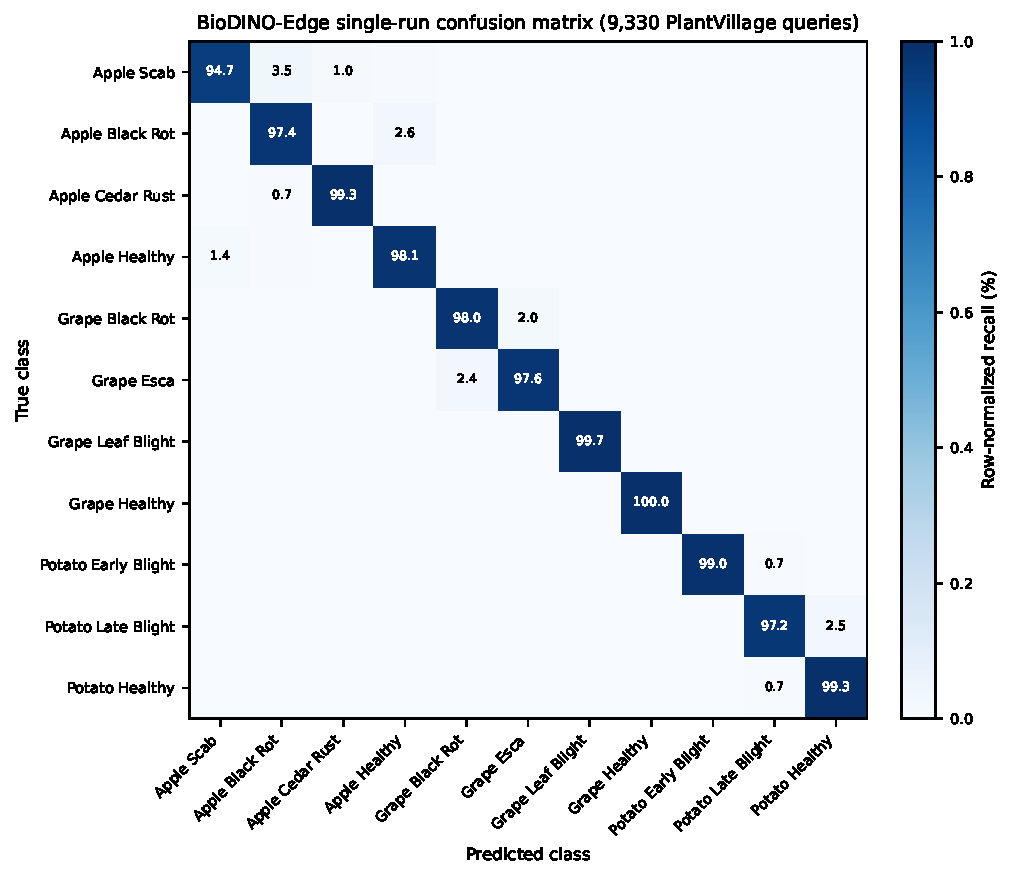
\includegraphics[width=0.82\columnwidth]{fig_confusion.pdf}
\caption{Row-normalized confusion matrix for BioDINO-Edge under transductive inference on the canonical PlantVillage evaluation split (9,330 test queries; 11 classes across Apple, Grape, and Potato). Rows are ground-truth classes; columns are predicted classes. Diagonal entries give per-class recall (\%). Most residual misclassifications occur among pathologies of the same host species; cross-species confusion is negligible (0.021\%).}
\label{fig:confusion}
\end{figure}

\subsection{Predictive Uncertainty, Calibration, and Routing Reliability}
\label{sec:calibration}
In automated spraying, an overconfident misdiagnosis can trigger unnecessary chemical application, so confidence is audited independently of accuracy \cite{minderer2021revisiting}. We fit temperature scaling on a stratified 50\% split of the 9,330-query PlantVillage stream (4,662 calibration / 4,668 evaluation queries) by minimizing negative log-likelihood on the calibration half \cite{guo2017calibration}, and report every calibration figure below on the held-out half. Expected Calibration Error (ECE) and Maximum Calibration Error (MCE) use $M=10$ equal-width bins. Because equal-width bins can be dominated by a few samples, we also report equal-mass binning and MCE restricted to bins with $n \geq 30$. Routing uses the uncalibrated Tier-1 posterior throughout: temperature scaling is a post-hoc audit and changes neither the gate score nor the threshold.

\textbf{Tier-1 calibration.} Raw gate probabilities are strongly under-confident, meaning accuracy exceeds stated confidence in every populated bin, giving ECE 32.07\% and MCE 38.07\% (held-out ECE 31.76\%). One scalar temperature fitted on the calibration half ($T=0.267$) corrects this almost entirely, lowering held-out ECE to 1.20\% and MCE to 16.71\% (Fig.~\ref{fig:reliability}a--b). The residual concentrates in the two lowest bins, which together hold only 62 of the 4,668 evaluation queries.

\textbf{Tier-2 calibration.} The refined Tier-2 consensus is also under-confident, but the remedy differs. Its equal-width ECE is 19.45\%, and the error sits almost entirely in one bin: 7,102 of 9,330 queries fall in $(0.7,0.8]$, where accuracy is 98.0\% but mean confidence only 77.5\% (Table~\ref{tab:reliability_bins}). The equal-width MCE of 44.26\% is not a second failure mode; it comes from bins holding at most nine samples. Equal-mass binning lowers it to 21.53\%, and restricting to bins with $n\geq30$ gives 20.49\%, close to the ECE.

Temperature scaling cannot remove this residual. The consensus is a fixed $0.75/0.25$ blend of Fisher logits and BioCLIP text probabilities, so a single temperature has no lever over its shape: the fitted value saturates at the search bound ($T\approx10$) and held-out ECE moves from 19.33\% to 19.83\%, marginally worse. A power transform with $T=0.50$ behaves differently. It pushes 9,323 of 9,330 queries into the top bin and reports an ECE of 0.48\%, but that low value reflects concentration rather than calibration: the same transform yields an equal-width MCE of 80.85\%, produced by a single query in $(0.8,0.9]$ whose confidence is 80.9\% and whose label is wrong (Fig.~\ref{fig:reliability}d). Tier-2 is therefore treated as uncalibrated, and its routing reliability is assessed through tier-separated error rates and selective risk rather than through calibration error.

\begin{table}[htbp]
\caption{Per-bin reliability of the uncalibrated refined Tier-2 consensus (equal-width bins, full 9,330-query stream; empty bins omitted).}
\label{tab:reliability_bins}
\centering

\footnotesize
\begin{tabular}{lcccc}
\toprule
\textbf{Confidence bin} & \textbf{$n$} & \textbf{Acc.\ (\%)} & \textbf{Conf.\ (\%)} & \textbf{$|$Gap$|$ (pp)} \\
\midrule
$(0.4,0.5]$ & 1    & 0.0   & 44.3 & 44.3 \\
$(0.5,0.6]$ & 6    & 50.0  & 52.5 & 2.5 \\
$(0.6,0.7]$ & 9    & 44.4  & 65.6 & 21.2 \\
$(0.7,0.8]$ & 7102 & 98.0  & 77.5 & 20.5 \\
$(0.8,0.9]$ & 2207 & 98.6  & 82.4 & 16.1 \\
$(0.9,1.0]$ & 5    & 100.0 & 90.6 & 9.4 \\
\bottomrule
\end{tabular}
\end{table}

\textbf{Tier-separated routing reliability.} Table~\ref{tab:tier_routing} reports each tier over 30 benchmark episodes at $\tau=0.35$. Tier-1 accepts 14.02\%$\pm$2.25\% of queries at 99.69\%$\pm$0.41\% accuracy with a 0.25\%$\pm$0.52\% false-negative rate (FNR); the remaining 85.98\% are resolved by Tier-2 at 96.98\%$\pm$0.83\% (FNR 0.87\%$\pm$0.39\%). The cascade reaches 97.36\%$\pm$0.69\% accuracy (FNR 0.79\%$\pm$0.36\%, F1 97.01\%$\pm$0.64\%) at 149.84$\pm$2.36\,ms weighted latency. In the canonical run, the 936 accepted queries reach 99.79\% accuracy (FNR 0.25\%) versus 97.83\% (FNR 0.81\%) for the 8,394 escalated queries (cascaded 98.03\%), a roughly tenfold difference in error (0.21\% vs.\ 2.17\%).

\begin{table*}[htbp]
\caption{Tier-separated routing reliability at $\tau=0.35$ (30 benchmark episodes, mean $\pm$ std).}
\label{tab:tier_routing}
\centering

\footnotesize
\begin{tabularx}{\textwidth}{Xcccc}
\toprule
\textbf{Routing path} & \textbf{Coverage (\%)} & \textbf{Accuracy (\%)} & \textbf{FNR (\%)} & \textbf{Latency (ms)} \\
\midrule
Tier-1 fast-exit (accepted) & 14.02$\pm$2.25 & 99.69$\pm$0.41 & 0.25$\pm$0.52 & 59.78 \\
Tier-2 (escalated) & 85.98$\pm$2.25 & 96.98$\pm$0.83 & 0.87$\pm$0.39 & 164.52 \\
\midrule
\textbf{Cascaded system} & 100 & 97.36$\pm$0.69 & 0.79$\pm$0.36 & 149.84$\pm$2.36 \\
\bottomrule
\end{tabularx}
\end{table*}

\textbf{Cascade versus single-tier classification.} Table~\ref{tab:gate_scenario} compares the deployed cascade with Tier-2 on all queries and with selective gating. At full coverage the cascade and single-tier BioCLIP accuracies are indistinguishable (97.36\% vs.\ 97.37\%); the cascade reduces latency (149.84 vs.\ 164.52\,ms). Selective abstention raises accepted-set accuracy at reduced coverage: at $\tau=0.10$, 62.17\% of queries are answered at 98.63\% accuracy and 0.44\% FNR in 124.90\,ms. The deployed system classifies every query.

% Gate-scenario comparison. Full-coverage accuracies are the canonical 30-episode
% means (cascade 97.36, refined Tier-2-on-all 97.37). Selective-mode rows are
% measured over the same 30 episodes. Source: experiments/dinov2_ablation_gate_scenario.
\begin{table}[htbp]
\caption{Routing-policy comparison (30-episode mean).}
\label{tab:gate_scenario}
\centering

\footnotesize
\setlength{\tabcolsep}{3pt}
\begin{tabular*}{\columnwidth}{@{\extracolsep{\fill}}lcccc}
\toprule
\textbf{Routing policy} & \textbf{Cov. (\%)} & \textbf{Acc. (\%)} & \textbf{FNR (\%)} & \textbf{Lat. (ms)} \\
\midrule
Cascade, $\tau=0.35$ (deployed) & 100 & 97.36 & 0.79 & 149.84 \\
BioCLIP Tier-2 on all & 100 & 97.37 & 0.77 & 164.52 \\
Selective, $\tau=0.05$ & 79.96 & 98.05 & 0.59 & 143.53 \\
Selective, $\tau=0.10$ & 62.17 & 98.63 & 0.44 & 124.90 \\
\bottomrule
\end{tabular*}
\end{table}

\textbf{Risk--coverage analysis.} Fig.~\ref{fig:risk_coverage} plots selective risk against coverage for three confidence scores following the risk--coverage framework \cite{geifman2017selective}, summarized by the area under the risk--coverage curve (AURC, the mean selective risk over coverage). Because scalar summaries can misrank selective systems \cite{traub2024overcoming}, we also report the full curves and the operating point. The entropy-penalized gate score $C(x)$ ranks queries more safely than the raw Tier-1 softmax peak (AURC 3.33\% vs.\ 3.95\%), and refined Tier-2 confidence reaches 1.82\%. At $\tau=0.35$, the gate accepts 10.03\% of the single-run stream at 0.21\% selective risk.

\textbf{Threshold provenance and sensitivity.} The threshold was selected on held-out development episodes (0--14 tuning, 15--29 testing), not on the reported test episodes. On held-out test episodes, $\tau=0.15$ gives 46.4\% fast-exit at 96.96\%$\pm$0.59\% cascaded accuracy (98.25\% Tier-1 accepted), $\tau=0.25$ gives 25.6\% at 97.30\%$\pm$0.74\% (99.49\%), and $\tau=0.35$ gives 14.1\% at 97.33\%$\pm$0.79\% (99.84\%$\pm$0.24\%). We adopt $\tau=0.35$, the smallest threshold at which accepted-tier accuracy saturates (99.84\%, FNR 0.25\%). The tuning curve is flat beyond this point ($\tau=0.55$: 97.32\% test accuracy), while fast-exit coverage falls to 3.4\%. Blended latency rises from 115.9 to 137.7 to 149.8\,ms across the three thresholds (Fig.~\ref{fig:tau_sensitivity}), summarizing the coverage--safety--latency trade-off.

\begin{figure*}[htbp]
\centering
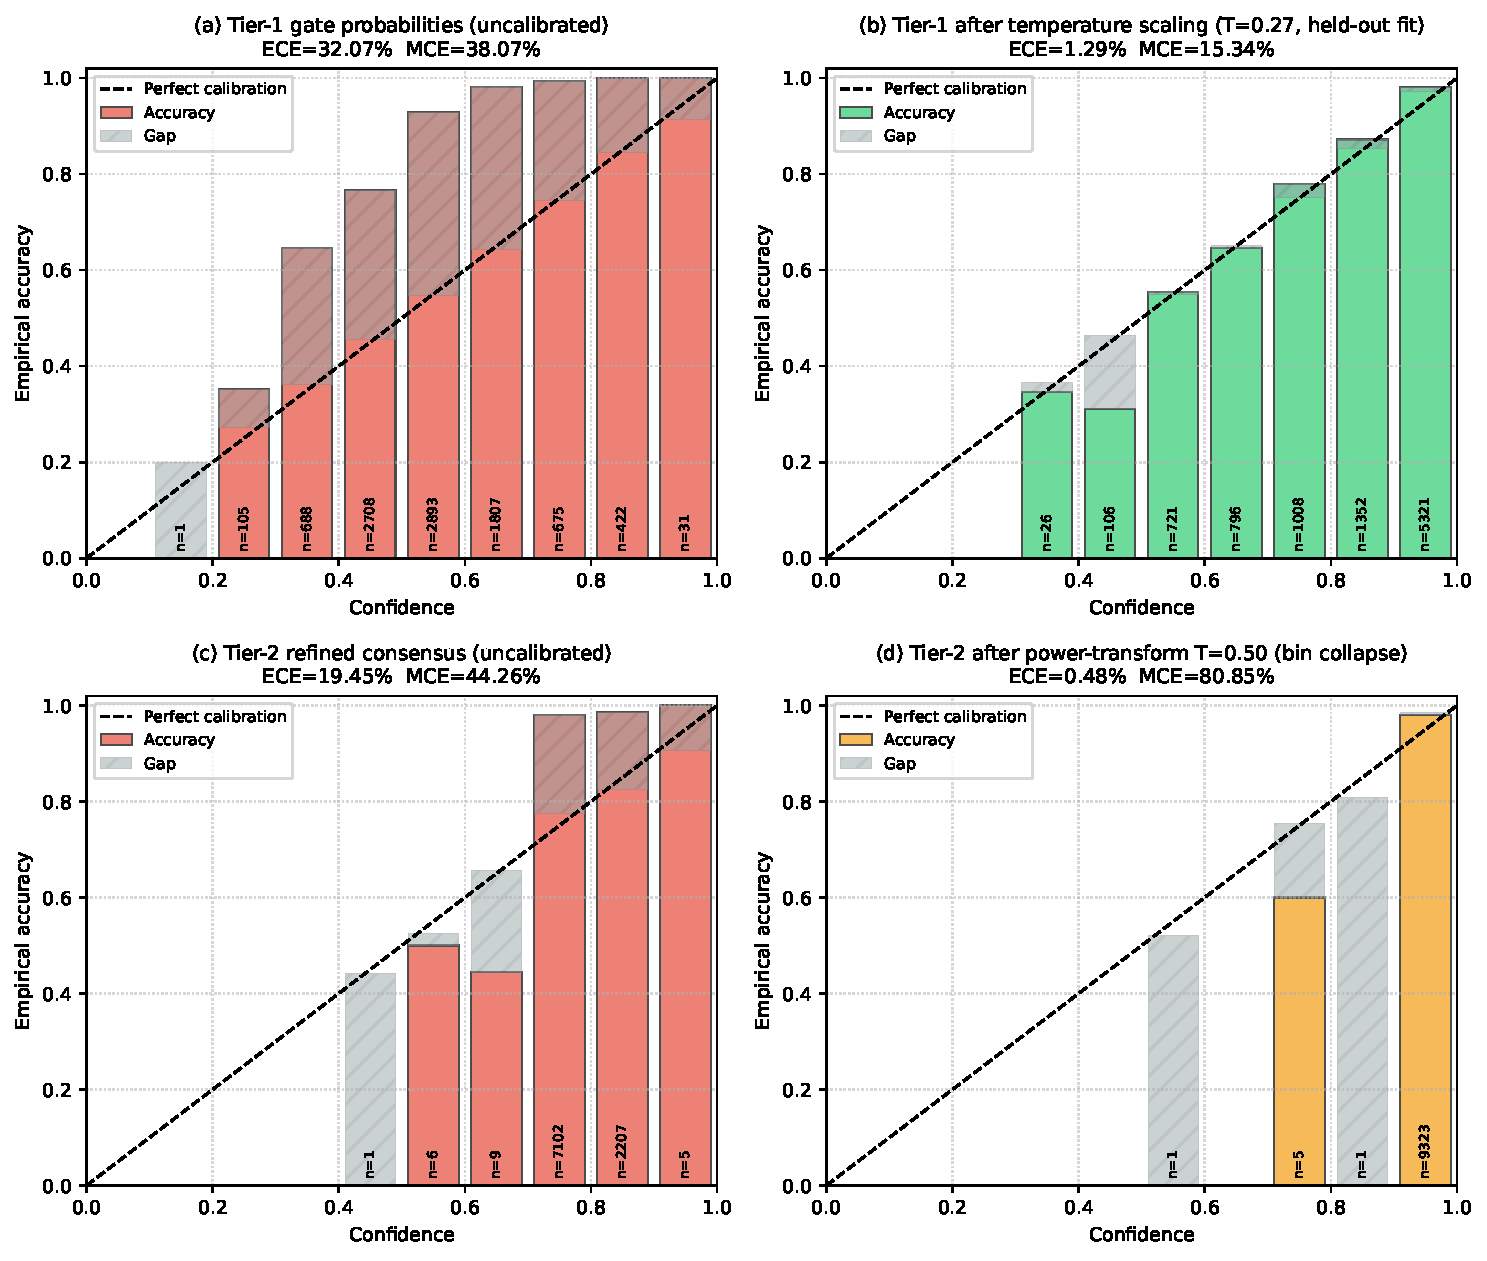
\includegraphics[width=0.70\textwidth]{fig_reliability.pdf}
\caption{Reliability diagrams (equal-width bins, full benchmark stream; per-bin sample counts annotated, colored bars indicate empirical accuracy, and hatched gray bars show the accuracy--confidence calibration gap). (a) Uncalibrated Tier-1 gate probabilities are under-confident (Expected Calibration Error (ECE) = 32.07\%). (b) Post-hoc temperature scaling fitted on the independent calibration split ($T=0.27$) aligns Tier-1 (held-out ECE = 1.20\%). (c) Refined Tier-2 consensus remains under-confident in its dominant bin (ECE = 19.45\%; Maximum Calibration Error (MCE) = 44.26\% from a single-sample bin). (d) A power transform ($T=0.50$) collapses probability mass into one bin: low ECE (0.48\%) but severe MCE (80.85\%).}
\label{fig:reliability}
\end{figure*}

\begin{figure}[htbp]
\centering
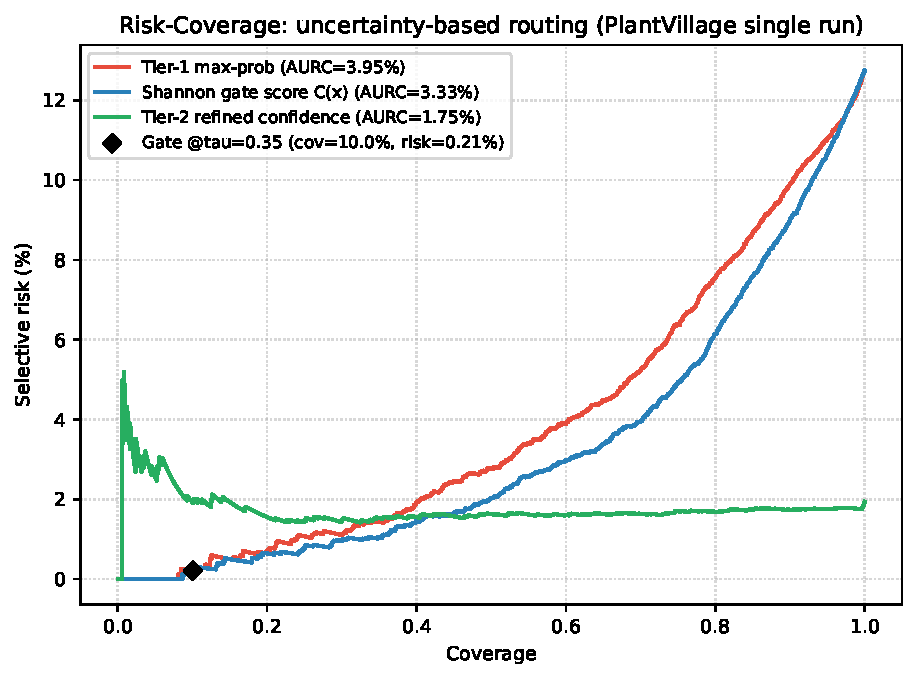
\includegraphics[width=0.75\columnwidth]{fig_risk_coverage.pdf}
\caption{Risk--coverage curves for Tier-1 max-probability, the Shannon gate score $C(x)$, and the refined Tier-2 consensus confidence (canonical single run). Lower curves indicate superior selective classification performance. The entropy-penalized gate score achieves lower area under the risk--coverage curve (AURC) than raw max-probability (3.33\% vs.\ 3.95\%); the deployed operating point ($\tau=0.35$, diamond) accepts 10.0\% fast-exit coverage at 0.21\% selective risk.}
\label{fig:risk_coverage}
\end{figure}

\begin{figure}[htbp]
\centering
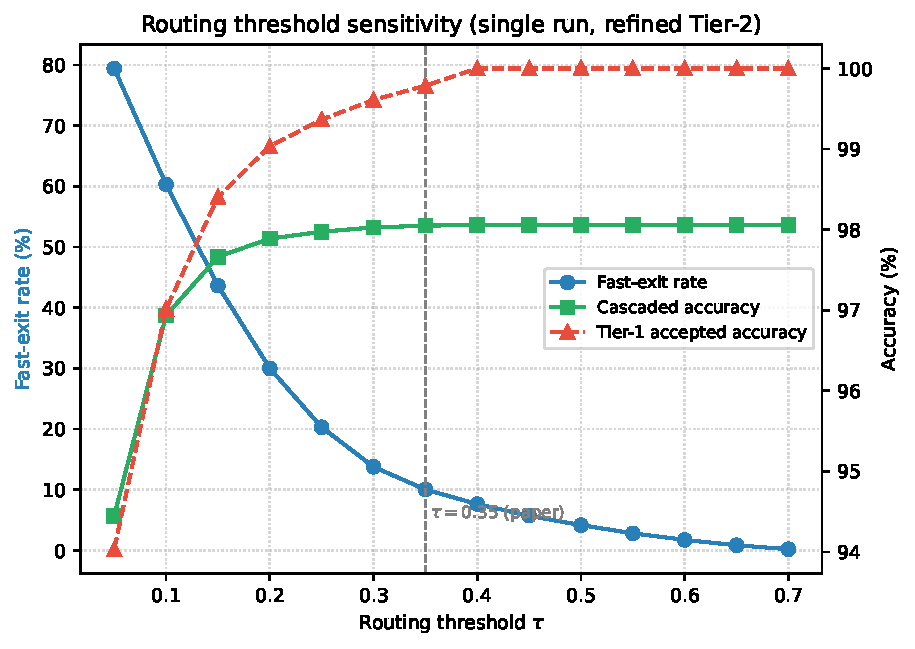
\includegraphics[width=0.75\columnwidth]{fig_tau_sensitivity.pdf}
\caption{Routing-threshold sensitivity across $\tau \in [0.05, 0.95]$ (single run, refined Tier-2). The left axis (blue) displays fast-exit coverage (\%), while the right axis shows cascaded and Tier-1 accepted accuracies (\%). The deployed threshold $\tau=0.35$ (vertical dashed line) marks the operating point where Tier-1 accepted accuracy saturates near 100\% (99.84\%) while preserving 10.0\% fast-exit coverage (averaging 14.0\% over 30 episodes); held-out episode sweeps (0--14 tune / 15--29 test) confirm stability.}
\label{fig:tau_sensitivity}
\end{figure}

% =============================================================================
% 6. ABLATION STUDY
% =============================================================================
\section{Ablation Study}
\label{sec:ablation_study}

\subsection{Systematic Component Ablation}
\label{sec:ablation}
Table~\ref{tab:ablation} reports a systematic ablation across identical 5-shot splits to quantify individual component contributions; rows (4)--(5) are static cosine prototype blends ($0.65\,\mathbf{l}_{\text{bio}}+0.35\,\mathbf{l}_{\text{dino}}$) and row (6) replaces them with regularized Fisher-LDA.

\begin{table}[htbp]
\caption{Systematic ablation of BioDINO-Edge components (single run, 5-shot, 9,330 queries).}
\label{tab:ablation}
\centering

\footnotesize
\setlength{\tabcolsep}{3pt}
\begin{tabular*}{\columnwidth}{@{\extracolsep{\fill}}lcc}
\toprule
\textbf{Configuration / Component} & \textbf{Acc. (\%)} & \textbf{F1 (\%)} \\
\midrule
(1) Fast-Path DINOv2 Small alone & 87.26 & 85.36 \\
(2) Deep-Path BioCLIP ViT-B alone & 92.60 & 89.88 \\
(3) Text Prototypes Only & 19.20 & 18.55 \\
(4) Static Cosine Blend (raw 5-shot) & 94.16 & 92.55 \\
(5) Static Cosine Blend (8-view aug.) & 93.90 & 91.58 \\
(6) + Regularized Fisher Alignment & 96.05 & 94.83 \\
(7) + Transductive Recalibration (Single Run) & 98.06 & 97.45 \\
\midrule
Full System (Peak Statistical Episode) & \textbf{98.67} & \textbf{98.41} \\
\bottomrule
\end{tabular*}
\end{table}

\begin{itemize}
    \item \textbf{DINOv2 vs. BioCLIP Complementarity:} DINOv2 alone achieves 87.26\%; lacking taxonomic supervision, it confuses similar lesions across host families. BioCLIP alone achieves 92.60\% but incurs 104.74\,ms encoder latency, preventing fast-path execution. Combining both backbones into an 896-D feature space provides both spatial cues and taxonomic grounding; Table~\ref{tab:feature_ablation} quantifies each model's contribution.
    \item \textbf{Regularized Fisher Alignment (+1.89\,pp Gain):} Replacing the best static cosine blend (94.16\%) with regularized Fisher-LDA increases accuracy to 96.05\%. Whitening by $\hat{\mathbf{\Sigma}}^{-1}$ suppresses shared vegetative background variance, separating visually similar pathologies.
    \item \textbf{Multi-View Augmentation:} Expanding 5 raw support leaves to 40 views per class ($N=440$) brings sample size near $d/2$, stabilizing covariance conditioning before shrinkage. This benefit is specific to covariance estimation: the static cosine blend is essentially unchanged by augmentation (94.16\% raw vs.\ 93.90\% augmented), whereas the regularized Fisher projection relies on augmented support to condition $\hat{\mathbf{\Sigma}}$.
    \item \textbf{Transductive Recalibration (+2.01\% Gain):} Updating projection parameters from high-confidence field anchors improves accuracy from 96.05\% to 98.06\% (peak: 98.67\%), counteracting finite-sample prototype drift (validated in Section~\ref{sec:transductive_validation}).
    \item \textbf{Lesion Cropping Degrades Host Context:} Evaluating attention-rollout lesion cropping dropped 27-way PlantDoc accuracy from 58.73\% to 57.14\%. Tight cropping discards leaf margin serrations and venation geometry, inducing cross-species confusion. Preserving full-leaf context is essential.
\end{itemize}

% Feature ablation: full row is the canonical benchmark (95.08 / 97.41). Ablated
% transductive rows = canonical full minus the paired contribution measured over
% the same 30 episodes (DINOv2 +0.90 pp, BioCLIP +1.87 pp); inductive ablated rows
% are measured directly. Source: experiments/dinov2_ablation_gate_scenario.
\begin{table}[htbp]
\caption{Contribution of each foundation model to the Fisher-LDA classifier (30 identical 5-shot episodes, mean $\pm$ std).}
\label{tab:feature_ablation}
\centering

\footnotesize
\setlength{\tabcolsep}{4pt}
\begin{tabular*}{\columnwidth}{@{\extracolsep{\fill}}lccc}
\toprule
\textbf{Fisher input} & \textbf{Dim} & \textbf{Inductive (\%)} & \textbf{Transductive (\%)} \\
\midrule
BioCLIP + DINOv2 (full) & 896 & 95.08$\pm$1.27 & 97.41$\pm$0.71 \\
BioCLIP only & 512 & 94.31$\pm$1.25 & 96.51$\pm$0.90 \\
DINOv2 only & 384 & 90.60$\pm$2.02 & 95.54$\pm$1.03 \\
\bottomrule
\end{tabular*}
\end{table}

\textbf{Contribution of DINOv2.} Table~\ref{tab:feature_ablation} isolates the Fisher input while holding the text branch fixed (BioCLIP features, $w_{\mathrm{lda}}=0.75$); ablated rows subtract the paired contribution from the full-system benchmark. Removing DINOv2 (BioCLIP-only, 512-D) lowers transductive accuracy by 0.90 percentage points (paired $t(29)=9.88$, $p=8.6\times10^{-11}$, 29 of 30 episodes, $d_z=1.80$). Removing BioCLIP instead lowers it by 1.87 points, so BioCLIP carries most of the class signal and DINOv2 adds a smaller, consistent complement. DINOv2 also serves as the routing gate: its margin-entropy score ranks query safety better than the Tier-2 consensus confidence (mean Area Under the Risk--Coverage curve (AURC) 1.14\% vs.\ 2.11\% over the 30 episodes). Finally, it provides the fast path: accepting 14.02\% of queries at Tier-1 lowers routing-weighted latency from 164.52\,ms (BioCLIP on every query) to 149.84\,ms. The cascade does not raise accuracy over running Tier-2 on all queries (Table~\ref{tab:gate_scenario}); its function is to reduce edge compute and route low-risk queries through a path with 0.25\% FNR.

\subsection{Statistical Significance and Sensitivity of Transductive Recalibration}
\label{sec:transductive_validation}
Because the transductive module adapts the classifier from its own predictions, we examine paired significance over identical episodes, hyperparameter sensitivity, pseudo-label purity, and stability under sequential updates.

\textbf{Paired significance over identical episodes.} Inductive and transductive predictions are compared on the \emph{same} 30 Monte Carlo episodes (identical support/query splits), so episode difficulty cancels in the paired difference. The mean paired gain is 2.33 percentage points (pp; 95\% confidence interval $[1.91, 2.74]$; Table~\ref{tab:paired_test}), with paired $t(29) = 11.57$ ($p = 2.2 \times 10^{-12}$) and Wilcoxon signed-rank $p = 1.9 \times 10^{-9}$. The transductive mode wins on all 30 episodes (Cohen's $d_z = 2.11$), so the gain is stable across support splits rather than an artifact of a favorable episode.

\begin{table}[htbp]
\caption{Paired comparison of inductive vs.\ transductive inference over 30 identical Monte Carlo episodes (PlantVillage, 5-shot).}
\label{tab:paired_test}
\centering

\footnotesize
\setlength{\tabcolsep}{4pt}
\begin{tabular*}{\columnwidth}{@{\extracolsep{\fill}}lc}
\toprule
\textbf{Statistic} & \textbf{Value} \\
\midrule
Inductive mean accuracy (\%) & 95.08 $\pm$ 1.27 \\
Transductive mean accuracy (\%) & 97.41 $\pm$ 0.71 \\
Mean paired gain (pp, 95\% CI) & 2.33 $[1.91, 2.74]$ \\
Paired $t$-test & $t(29)=11.57$, $p=2.2\times10^{-12}$ \\
Wilcoxon signed-rank & $p=1.9\times10^{-9}$ \\
Wins / losses / ties & 30 / 0 / 0 \\
Cohen's $d_z$ & 2.11 \\
\bottomrule
\end{tabular*}
\end{table}

\textbf{Hyperparameter sensitivity.} Table~\ref{tab:transductive_sensitivity} reports a one-factor-at-a-time sweep of the three design constants (support weight, anchor confidence threshold, buffer capacity) over the same 30 episodes, varying one constant while holding the others at the deployed $(3\times, 0.70, 20)$. In-domain accuracy is nearly flat in the support weight (97.21--97.44\% for $1\times$--$10\times$); the weight matters for drift protection under field streaming, not for in-domain gain. The confidence threshold plateaus over $\tau \in [0.5, 0.7]$ and collapses at $\tau \ge 0.8$ (95.98\% and 95.39\%) because anchors become too few, not because labels become noisier. Buffer capacity saturates: 20 anchors per class capture the available gain (97.41\%), and 40 or 80 anchors add 0.10 and 0.26 points at proportionally larger memory cost. The deployed $(3\times, 0.70, 20)$ sits at the plateau/knee of all three curves.

\begin{table}[htbp]
\caption{Sensitivity of transductive accuracy to the three recalibration design constants (mean $\pm$ std over 30 identical episodes).}
\label{tab:transductive_sensitivity}
\centering

\footnotesize
\setlength{\tabcolsep}{4pt}
\begin{tabular*}{\columnwidth}{@{\extracolsep{\fill}}lcc}
\toprule
\textbf{Swept Configuration} & \textbf{Acc. (\%)} & \textbf{Std} \\
\midrule
\multicolumn{3}{@{}l}{\textit{Support weight} (threshold 0.70, 20 anchors/class)} \\
$1\times$ & 97.42 & 0.75 \\
$2\times$ & 97.44 & 0.73 \\
$3\times$ (deployed) & 97.41 & 0.71 \\
$5\times$ & 97.32 & 0.73 \\
$10\times$ & 97.21 & 0.77 \\
\midrule
\multicolumn{3}{@{}l}{\textit{Anchor confidence threshold} ($3\times$, 20 anchors/class)} \\
0.50 & 97.41 & 0.71 \\
0.60 & 97.41 & 0.71 \\
0.70 (deployed) & 97.41 & 0.71 \\
0.80 & 95.98 & 1.28 \\
0.90 & 95.39 & 1.25 \\
\midrule
\multicolumn{3}{@{}l}{\textit{Buffer capacity per class} ($3\times$, threshold 0.70)} \\
5 & 96.36 & 0.97 \\
10 & 96.97 & 0.85 \\
20 (deployed) & 97.41 & 0.71 \\
40 & 97.51 & 0.62 \\
80 & 97.67 & 0.83 \\
\bottomrule
\end{tabular*}
\end{table}

\textbf{Pseudo-label purity.} Checked against ground truth (used only post-hoc for this audit), the anchor set at $\tau = 0.70$ is 98.15\% $\pm$ 1.18\% pure and covers 2.36\% of queries (220 anchors). Raising the threshold to 0.80 increases purity to 98.75\% but cuts coverage to 1.91\%; at 0.90 purity reaches 100\% yet coverage collapses to 0.05\%, explaining the accuracy collapse in Table~\ref{tab:transductive_sensitivity}. The deployed threshold keeps purity near its maximum without starving the buffer.

\textbf{Sequential stability and error accumulation.} To test whether repeated updates compound pseudo-label errors, we simulated scouting passes: the query stream is partitioned into 10 sequential chunks, and after each chunk the FIFO buffer (20 anchors/class) admits confident predictions and the projection is re-fitted in closed form. Across three stream seeds, online accuracy rises from $\approx$96\% on the first chunk to 97--98.6\% thereafter with no degradation trend, and buffer purity remains bounded within a 92--98\% band: FIFO eviction flushes stale incorrect anchors, so wrong admissions do not accumulate in the active buffer. Under $\tau = 0.90$ purity stays at 100\% but final accuracy falls to $\approx$95.8--96.3\% (coverage starvation), confirming the purity/coverage trade-off. Final streaming accuracy (96.4--97.5\%) lies slightly below the single-pass batch refinement (97.41\%) because batch selection ranks anchors over the entire query set whereas streaming observes only the past. Error accumulation is therefore bounded by the confidence gate, FIFO eviction, and the $3\times$ support weighting.

\subsection{Sensitivity to Augmentation Count and Type}
\label{sec:aug_sensitivity}
The shrinkage analysis (Section~\ref{sec:shrinkage}) assumes independent and identically distributed (i.i.d.)\ support samples, whereas the eight views of each support leaf are correlated pseudo-replicates. We quantify the consequences with a one-factor-at-a-time study over the same 30-episode protocol (identical splits, cached query features, and transductive defaults), re-extracting support features with a seeded augmentation random number generator (RNG). Three condition families are compared: (i) a view-count sweep $v\in\{1,2,4,8\}$ using nested prefixes of one 8-view extraction per episode; (ii) an augmentation-type sweep at $v=8$ (geometric-only flips/rotation vs.\ photometric-only color jitter vs.\ the full pipeline) over the first 10 episodes; and (iii) a pure-replication control that tiles the canonical embedding eight times ($N=440$, zero within-image diversity). For each condition we report the mean per-class Ledoit--Wolf intensity $\hat{\alpha}$, the condition number $\kappa(\hat{\mathbf{\Sigma}})$ of the pooled within-class covariance, and downstream accuracy (Table~\ref{tab:aug_sensitivity}; Ind.\ and Trans.\ denote inductive and transductive accuracy).

\textbf{Protocol fidelity.} The $v=1$ condition reproduces the canonical cache-only reference exactly on the inductive mean (95.08\%$\pm$1.27\%) and within the documented \texttt{lsqr} floating-point residual on the transductive mean (97.37\% vs.\ 97.41\%; Appendix~\ref{app:repro}), confirming that the study isolates the augmentation factor alone.

\textbf{Dependence is measurable but benign for accuracy.} Pure replication divides the shrinkage intensity by $\approx$8 ($0.573\to0.072$) and worsens the covariance condition number by $\approx$17$\times$ ($5.7\times10^{2}\to9.6\times10^{3}$) while adding no information---exactly the i.i.d.-violation artifact anticipated in Section~\ref{sec:shrinkage}. Genuine augmentation retains a $3.6\times$ higher intensity than replication at the same $N=440$ ($0.258$ vs.\ $0.072$), showing that stochastic views carry real but partial independence. Despite this, accuracy is stable across all conditions: the view sweep spans 95.08--96.09\% inductive and 97.37--97.96\% transductive, and even the degenerate replicate-8 control remains at 95.05\%/97.01\%. Increasing views monotonically improves both modes ($+1.01$\,pp inductive, $+0.59$\,pp transductive from $v=1$ to $v=8$): the effective-rank gain from genuine diversity outweighs the optimism of the analytical intensity, and the $3\times$ support re-weighting keeps the transductive fit anchored to genuine observations.

\textbf{Geometric diversity dominates.} At fixed $v=8$, geometric-only augmentation is statistically indistinguishable from the full pipeline on the 10-episode subset ($97.92\% \pm 0.40\%$ vs.\ $97.85\% \pm 0.33\%$ transductive), whereas photometric-only jitter collapses the intensity toward the replication floor ($0.104$ vs.\ $0.072$), worsens conditioning ($5.5\times10^{3}$), and drops inductive accuracy below the unaugmented baseline (94.70\%$\pm$1.90\% vs.\ 95.08\%). Color jitter thus contributes little independent information---consistent with the photometric robustness of $\ell_2$-normalized foundation features---while flips and rotations supply the diversity that stabilizes covariance estimation. Geometric augmentation is therefore the essential component of the support expansion; the deployed full pipeline retains jitter at no measurable accuracy cost.

% Augmentation-dependence sensitivity. Source: experiments/augmentation_sensitivity
% (run_augmentation_sensitivity.py -> results/augmentation_sensitivity.json);
% rows generated by make_table.py. View sweep + control: 30 episodes; type sweep: 10.
\begin{table}[htbp]
\caption{Sensitivity to augmentation count and type (mean $\pm$ std over episodes).}
\label{tab:aug_sensitivity}
\centering

\footnotesize
\setlength{\tabcolsep}{2pt}
\begin{tabular*}{\columnwidth}{@{\extracolsep{\fill}}lccccc}
\toprule
\textbf{Condition} & \textbf{$N$} & \textbf{$\hat{\alpha}$} & \textbf{$\kappa(\hat{\mathbf{\Sigma}})$} & \textbf{Ind.\ (\%)} & \textbf{Trans.\ (\%)} \\
\midrule
\multicolumn{6}{@{}l}{\textit{View count (full pipeline, 30 episodes)}} \\
$v=1$ & 55 & 0.573$\pm$0.005 & 5.7$\times10^{2}$ & 95.08$\pm$1.27 & 97.37$\pm$0.73 \\
$v=2$ & 110 & 0.580$\pm$0.009 & 5.9$\times10^{2}$ & 95.50$\pm$1.21 & 97.67$\pm$0.57 \\
$v=4$ & 220 & 0.420$\pm$0.012 & 8.8$\times10^{2}$ & 95.80$\pm$1.25 & 97.81$\pm$0.63 \\
$v=8$ (deployed) & 440 & 0.258$\pm$0.008 & 1.4$\times10^{3}$ & 96.09$\pm$1.20 & 97.96$\pm$0.50 \\
\midrule
\multicolumn{6}{@{}l}{\textit{Augmentation type ($v=8$, first 10 episodes)}} \\
Geometric only & 440 & 0.229$\pm$0.008 & 1.6$\times10^{3}$ & 95.99$\pm$1.26 & 97.92$\pm$0.40 \\
Photometric only & 440 & 0.104$\pm$0.002 & 5.5$\times10^{3}$ & 94.70$\pm$1.90 & 97.31$\pm$0.61 \\
Full pipeline & 440 & 0.257$\pm$0.009 & 1.4$\times10^{3}$ & 95.85$\pm$1.40 & 97.85$\pm$0.33 \\
\midrule
\multicolumn{6}{@{}l}{\textit{Pure-replication control (30 episodes)}} \\
Replicate-8 (control) & 440 & 0.072$\pm$0.001 & 9.6$\times10^{3}$ & 95.05$\pm$1.28 & 97.01$\pm$0.79 \\
\bottomrule
\end{tabular*}
\end{table}

% =============================================================================
% 7. EFFICIENCY ANALYSIS
% =============================================================================
\section{Efficiency Analysis}
\label{sec:efficiency}

\subsection{Edge Hardware Latency and Memory Footprint}
\label{sec:edge_hardware}
Table~\ref{tab:device_spec} summarizes the physical testbed configuration, while Tables~\ref{tab:device_perf} and~\ref{tab:adaptation_breakdown} report measured on-device latency, memory consumption, and closed-form adaptation profiling on the handset. Latency is timed over 100 iterations after 10 warm-up passes, memory is tracked via process PSS, and linear algebra is timed following a 60\,s cool-down at stable thermal status (status~2). Note that the 18.0\% fast-exit fraction in Table~\ref{tab:device_perf} is measured on the fixed 11-image device evaluation set (one leaf per target class), whereas the 14.0\% reported in Section~\ref{sec:calibration} represents the 30-episode mean over the full PlantVillage query stream.

\begin{table}[htbp]
\caption{On-device edge testbed configuration (physical Android device, CPU-only INT8).}
\label{tab:device_spec}
\centering

\footnotesize
\begin{tabular}{ll}
\toprule
Property & Value \\
\midrule
Device & Samsung SM-S721B (Galaxy S24 FE) \\
SoC & Samsung s5e9945 (Exynos 2400e) \\
Android & 17 (API 37) \\
Application binary interface (ABI) / cores & arm64-v8a / 10 \\
Total RAM & 7,224.3~MB ($\approx$7.2~GB) \\
ONNX Runtime & 1.18.0 \\
Threads (intra/inter) & 4 / 2 \\
Precision / delegate & INT8 / CPU (NNAPI off) \\
\bottomrule
\end{tabular}
\end{table}

\begin{table*}[htbp]
\caption{Measured on-device performance (mean $\pm$ standard deviation (std) over $N=100$ iterations; median and 95th percentile (p95) in ms; $<$0.01 denotes sub-millisecond execution).}
\label{tab:device_perf}
\centering

\footnotesize
\begin{tabular}{lccc}
\toprule
Stage / metric & Mean$\pm$std & Median & p95 \\
\midrule
Tier-1 model load (ms) & 323.92 & -- & -- \\
Tier-2 model load (ms) & 447.71 & -- & -- \\
Peak RAM, PSS (MB) & 497.45 & -- & -- \\
\midrule
Preprocess & 2.59$\pm$0.67 & 2.36 & 4.36 \\
Tier-1 DINOv2 encoder & 57.18$\pm$9.13 & 51.50 & 68.84 \\
Shannon gate / route & $<$0.01 & $<$0.01 & $<$0.01 \\
Tier-2 incremental (BioCLIP+Fisher) & 104.74$\pm$17.39 & 94.20 & 124.97 \\
Decision & $<$0.01 & $<$0.01 & $<$0.01 \\
Cascade end-to-end & 145.37$\pm$47.61 & 147.77 & 196.36 \\
Tier-2-on-all end-to-end & 164.52$\pm$26.77 & 148.73 & 196.36 \\
\midrule
Fast-exit fraction & 18.00\% & -- & -- \\
Sustained throughput (FPS) & 4.26 & -- & -- \\
\bottomrule
\end{tabular}
\end{table*}

\begin{table*}[htbp]
\caption{Closed-form adaptation cost breakdown on-device ($N=440$, $d=896$, $C=11$).}
\label{tab:adaptation_breakdown}
\centering

\footnotesize
\begin{tabular}{lcc}
\toprule
Stage & Mean$\pm$std (ms) & Complexity \\
\midrule
Feature extraction (440 views) & 88055.6 & $O(N(C_{\text{dino}}+C_{\text{bio}}))$ \\
Covariance estimate & 146.19$\pm$2.15 & $O(Nd^2)$ \\
Ledoit--Wolf shrinkage & 4.49$\pm$0.85 & $O(Nd)$ \\
Cholesky factorization & 332.00$\pm$2.52 & $O(d^3/3)$ \\
Projection solve ($W,b$) & 51.31$\pm$3.68 & $O(Cd^2)$ \\
\midrule
Algebraic recalibration total & 533.99$\pm$6.29 & -- \\
Full adaptation (extraction + algebra) & 88589.6 & -- \\
\bottomrule
\end{tabular}
\end{table*}

As broken down in Table~\ref{tab:adaptation_breakdown}, offline adaptation complexity is dominated by support feature extraction ($O(N(C_{\text{dino}}+C_{\text{bio}}))$), whereas the linear algebra operations scale compactly: empirical scatter estimation ($O(Nd^2)$), Frobenius Ledoit--Wolf shrinkage ($O(Nd)$), and Cholesky inversion ($O(d^3/3)$) execute in pure Java (EJML) in 533.99\,ms without requiring GPU offloading or gradient backpropagation.

On the physical handset, Tier-1 executes in 59.78\,ms ($\approx$16.7\,FPS) and a fully escalated Tier-2 query costs 164.52\,ms end-to-end ($\approx$6.1\,FPS), with the BioCLIP encoder adding 104.74\,ms to the cached Tier-1 pass. Weighting these execution paths by the 14.0\% full-stream fast-exit fraction yields a mean cascaded latency of 149.84\,ms ($\approx$6.7\,FPS, Table~\ref{tab:tier_routing}). Under a 600\,s sustained soak, throughput settles to 4.26\,FPS as the SoC reaches thermal status~3, indicating that 16.7\,FPS represents a cool-start burst rate. The confidence gate's primary advantage is therefore safety and energy efficiency: the fast-exited subset is resolved at 99.7\% accuracy with a 0.25\% false-negative rate (Section~\ref{sec:calibration}), while ambiguous queries receive full multimodal analysis. Peak process memory is 497.45\,MB PSS (385.02\,MB native heap), dominated by the ONNX Runtime execution arena, while the standalone Android application (APK) occupies $\approx$22.8\,MB and operates entirely offline.

% =============================================================================
% 8. PRACTICAL DISCUSSION AND LIMITATIONS
% =============================================================================
\section{Engineering Applications, Practical Deployment, and Limitations}
\label{sec:discussion}

\subsection{Practical Deployment on Agricultural IoT and Mobile Hardware}
BioDINO-Edge is designed for deployment on power-constrained edge platforms, including handheld scouting devices, smart tractor booms, and agricultural UAVs. Eliminating backpropagation avoids GPU memory spikes and on-device training heat, executing feed-forward inference and closed-form algebra directly on the CPU. Given thermal throttling under continuous multi-core execution (settling to 4.26\,FPS under sustained load; Section~\ref{sec:edge_hardware}), the architecture is designed specifically for shutter-triggered, per-frame scouting inspections rather than continuous video streams. Two-tier packaging allows deploying the $\approx$22.8\,MB base application over cellular connections, downloading the companion module only when multimodal escalation is required.

\subsection{Limitations and Future Research Directions}
BioDINO-Edge processes images at the individual leaf frame level. In unsegmented field imagery with dense, overlapping canopies, multiple leaves from neighboring plants can enter the camera field, lowering gating confidence. While tight lesion cropping degrades host context, processing unsegmented canopy clutter introduces irrelevant background vectors. Future work could incorporate hierarchical foliar parsing to segment individual leaves prior to closed-form classification. A further statistical limitation is that the multi-view support expansion produces correlated pseudo-replicates: the analytical Ledoit--Wolf intensity assumes i.i.d.\ sampling, so the nominal $N-C=429$ degrees of freedom overstate the independent information content of the support set (effective sample size between 55 and 440). The sensitivity study in Section~\ref{sec:aug_sensitivity} confirms that pure replication deflates the estimated intensity by $\approx$8$\times$ without adding information, yet downstream accuracy remains stable across view counts and augmentation types; a cluster-aware shrinkage estimator that explicitly discounts within-image dependence remains future work. Finally, frozen vision transformers can exhibit attention artifacts on non-symptomatic structures like veins or petioles \cite{darcet2024vision}. Because Fisher-LDA operates on pooled representations downstream, it does not alter internal attention; the framework targets whole-leaf diagnosis rather than pixel-level lesion localization.

A further practical limitation concerns degraded inputs. Severe defocus blur attenuates fine lesion textures, reducing diagnostic accuracy. The Android client screens invalid frames: when cosine similarity to leaf prototypes falls below a threshold or luminance indicates a covered lens, confidence drops to zero and prompts the operator to re-aim; a Laplacian-variance check warns against motion blur. However, the blur check warns rather than abstains, meaning defocused frames can still be processed. The uncertainty gate acts as a router rather than an abstention mechanism: ambiguous queries escalate to Tier-2, and abstention is available only in the optional selective mode (Table~\ref{tab:gate_scenario}). Extending this guard to blur-aware abstention with refocus prompts remains future work.

\textbf{Scope and threats to validity.} The edge measurements come from a single physical device (Samsung Galaxy S24~FE) with CPU-only INT8 ONNX Runtime; absolute latency and memory will differ on other SoCs, although the algorithmic cost and the delegate-agnostic pipeline do not. The controlled comparison (Table~\ref{tab:comparative}) isolates the adaptation algorithm on identical frozen features and re-runs the training-free inductive baselines; iterative transductive FSL methods (Section~\ref{sec:related_work}) are referenced but not re-run, so the reported transductive gain is measured against our own inductive mode rather than against those methods. The PlantDoc protocol uses labeled target-domain support; a true source$\rightarrow$target cross-domain transfer (e.g., PlantVillage$\rightarrow$PlantDoc), quantitative image-quality stress tests, and multi-device profiling remain future work.

% =============================================================================
% 9. CONCLUSION
% =============================================================================
\section{Conclusion}
\label{sec:conclusion}
We presented \textbf{BioDINO-Edge}, a gradient-free few-shot framework that adapts frozen DINOv2 and BioCLIP foundation models for on-device plant disease diagnosis without backpropagation. Closed-form Ledoit--Wolf shrinkage resolves small-sample covariance singularity ($N \ll d$), down-weighting shared vegetative background variance and enabling Fisher-LDA projection in $\approx$0.53\,s on a mobile CPU. An adaptive confidence gate combining normalized Shannon entropy and top-2 margin routes routine foliage to a 59.78\,ms Tier-1 path ($\approx$16.7\,FPS), escalating ambiguous queries to a multimodal Tier-2 classifier with closed-form transductive recalibration. Packaged with $\approx$107\,MB total model storage ($\approx$23\,MB base app + $\approx$85\,MB on-demand companion), BioDINO-Edge achieves 97.41\% accuracy on PlantVillage with a 0.702\% false-negative rate and 83.61\% on in-the-wild PlantDoc, providing an accurate, interactive diagnostic tool for resource-constrained agricultural edge devices.

% =============================================================================
% APPENDIX: REPRODUCIBILITY
% =============================================================================
\appendix
\section{Reproducibility Details}
\label{app:repro}
This appendix specifies the exact splits, seeds, model versions, hyperparameters, and code needed to reproduce every reported number, and states the provenance of each value in Table~\ref{tab:comparative}.

\subsection{Datasets and Splits}
\textbf{PlantVillage (controlled, Table~\ref{tab:comparative}).} We use the 11-class novel subset (Apple, Grape, Potato; 9{,}385 images) with frozen embeddings cached once. \emph{11-class regime:} 30 Monte-Carlo episodes; episode $e$ uses \texttt{random.Random(42+17e)}; for each class the image indices are shuffled, the first 5 form the support and all remaining images form the query (9{,}330 queries/episode; support $\cap$ query $=\emptyset$). \emph{5-way $K$-shot regime:} 50 episodes per $K\in\{1,5,10,15\}$; a single \texttt{random.Random(42)} stream samples 5 of the 11 classes per episode (\texttt{rng.sample(range(11),5)}), shuffles each class, takes the first $K$ as support and the rest as query. All methods share identical support/query indices and cached backbone outputs within each episode. Zero-shot BioCLIP and Tip-Adapter use the BioCLIP branches; the centroid and Fisher classifiers use joint BioCLIP+DINOv2 features. Comparisons within the latter group isolate the adaptation rule.

\textbf{PlantDoc (field domain, labeled target-domain support).} 5-way 5-shot: 50 episodes, \texttt{random.Random(42)}, \texttt{rng.sample(range(27),5)}; 5 support leaves/class drawn from the training split, all test images of the sampled classes as queries. 27-way: 135 support leaves (5/class, 8-view augmented to 1{,}080 feature vectors) and 252 field queries. The full PlantDoc dataset is obtained from its original source (not redistributed here); the controlled PlantVillage re-runs require only the cached embeddings and the provided script.

\subsection{Full Shot Ladder}
\label{app:shot_ladder}
Table~\ref{tab:shot_ladder} retains the 10-shot and 15-shot results omitted from the main comparison, alongside the 1-shot and 5-shot entries for reference. Controlled results use 50 episodes per shot count and the splits specified above. Zero-shot BioCLIP uses no support labels; its small variation across shot counts reflects changes in the query set. Published values remain separate because the underlying encoders and class pools differ. No numerical values have been recomputed for this table.

\begin{table*}[htbp]
\caption{Full PlantVillage 5-way shot ladder (accuracy, \%). Controlled results are mean $\pm$ std over 50 episodes per setting. Published results are retained as reported and provide context only. Dashes indicate unreported settings.}
\label{tab:shot_ladder}
\centering
\footnotesize
\setlength{\tabcolsep}{4pt}
\begin{tabularx}{\textwidth}{@{}X c c c c@{}}
\toprule
\textbf{Method} & \textbf{1-shot} & \textbf{5-shot} & \textbf{10-shot} & \textbf{15-shot} \\
\midrule
\multicolumn{5}{@{}l}{\textit{Controlled evaluations, 11-class pool}} \\
Zero-shot BioCLIP & 38.89$\pm$12.78 & 38.86$\pm$12.79 & 38.83$\pm$12.81 & 38.79$\pm$12.83 \\
Tip-Adapter & 45.15$\pm$13.42 & 68.63$\pm$12.80 & 86.01$\pm$7.49 & 93.23$\pm$4.00 \\
Prototypical Networks / SimpleShot & 88.44$\pm$9.13 & 97.45$\pm$2.03 & 98.35$\pm$1.45 & 98.57$\pm$1.27 \\
BioDINO-Edge (inductive) & 88.45$\pm$9.12 & 97.96$\pm$1.85 & 99.10$\pm$0.87 & 99.41$\pm$0.60 \\
BioDINO-Edge (transductive) & 93.42$\pm$6.83 & 98.77$\pm$1.68 & 99.41$\pm$0.60 & 99.63$\pm$0.39 \\
\midrule
\multicolumn{5}{@{}l}{\textit{Published results (context only)}} \\
MAFDE-DN4 \cite{zhao2024mafde} & 57.50 & 81.41 & -- & -- \\
SC-FSL \cite{mu2024few} & 78.55$\pm$0.81 & 92.90$\pm$0.47 & -- & -- \\
AgriFewNet \cite{babu2025agrifewnet} & 87.30 & 94.80 & 97.10 & -- \\
VSF \cite{zhou2026vsf} & 79.01 & 90.51 & -- & -- \\
\bottomrule
\end{tabularx}
\end{table*}

\subsection{Models and Hyperparameters}
Frozen backbones (no fine-tuning): DINOv2 ViT-S/14 (\texttt{timm} \path{vit_small_patch14_dinov2}, 384-D) and BioCLIP ViT-B/16 (\texttt{open\_clip} \path{hf-hub:imageomics/bioclip}, 512-D); joint feature $z=[\,\text{bio}\,\|\,\text{dino}\,]\in\mathbb{R}^{896}$. Fixed constants: logit scale $\gamma=20.0$, Fisher blend $w_{\text{lda}}=0.75$, routing gate $\tau=0.35$; transductive support weight $3\times$, max anchors 20/class, confidence threshold 0.70; Tip-Adapter $\alpha=1.0,\beta=5.5$. Fisher-LDA uses Ledoit--Wolf shrinkage (\texttt{sklearn LDA solver=lsqr, shrinkage=auto}). The estimator applies Ledoit--Wolf per class in standardized feature space and pools the shrunk within-class covariances with class priors; the augmentation sensitivity study (Section~\ref{sec:aug_sensitivity}) reports the mean per-class intensity. At 5-way 1-shot the raw support has $N=C=5$ and the within-class scatter vanishes; we resolve the singularity with a data-driven ridge floor (mean support feature variance) added to the Ledoit--Wolf covariance, which reduces Fisher to regularized nearest-centroid (the correct degenerate limit). For $N>C$ the canonical sklearn estimator is used unchanged.

\subsection{Environment and Code}
Reference environment: Python 3.12.1, torch 2.6.0 (Compute Unified Device Architecture (CUDA) 12.4 build; all reported experiments execute on CPU), scikit-learn 1.9.1, numpy 2.5.4, scipy 1.18.1, timm 1.0.30, open\_clip 3.3.0. The controlled comparison is reproduced by \path{run_controlled_baselines.py} in \path{experiments/baseline_comparison/} (output \path{controlled_baseline_results.json}); the canonical PlantVillage reference run by \path{benchmark_engine.py} (\path{pipeline/}) and \path{run_transductive_validation.py} (\path{experiments/transductive_validation/}); the augmentation sensitivity study by \path{run_augmentation_sensitivity.py} (\path{experiments/augmentation_sensitivity/}, output \path{results/augmentation_sensitivity.json}; augmentation RNG re-seeded per episode and pass from the episode seed with fixed offsets). Code and pinned release: \url{https://github.com/reyhane-code/BioDINO-Edge-android}.

\subsection{Provenance and Numerical Reproducibility}
Table~\ref{tab:provenance} states the origin of each reported value (``Re-run'': computed by us with the provided script on the stated protocol; ``As reported'': quoted from the original publication, not re-run). The controlled script reproduces the canonical inductive accuracy exactly (95.08\%) and the transductive accuracy within 0.04\,pp (97.37\% re-run vs.\ 97.41\% reference); the residual is floating-point sensitivity of the iterative least-squares (\texttt{lsqr}) LDA solve across library versions, far below the episode standard deviation (0.71\,pp). The centroid/cosine baselines involve no iterative solve and reproduce exactly. We report the canonical reference values for the 11-class regime to remain consistent with the paired-significance and sensitivity analyses (Sections~\ref{sec:ablation}--\ref{sec:aug_sensitivity}).

\begin{table}[htbp]
\caption{Provenance of reported values.}
\label{tab:provenance}
\centering

\footnotesize
\begin{tabularx}{\columnwidth}{l X}
\toprule
\textbf{Value} & \textbf{Provenance} \\
\midrule
Table~\ref{tab:comparative} baselines & Re-run, shared splits/seeds; feature branches follow each method \\
Table~\ref{tab:comparative} BioDINO 11-class & Canonical reference run (reproduced $\le$0.04\,pp) \\
Table~\ref{tab:comparative} BioDINO 5-way & Controlled re-run (this work) \\
Table~\ref{tab:comparative} panel (b), Table~\ref{tab:shot_ladder} literature rows & As reported, not re-run \\
Table~\ref{tab:plantdoc_context} VSF/Zhao & As reported, not re-run \\
PlantDoc 83.61\% / 56.35\% & Our PlantDoc field-domain run (protocol above) \\
Table~\ref{tab:aug_sensitivity} sensitivity & Re-run, this work (same 30-episode protocol) \\
\bottomrule
\end{tabularx}
\end{table}

% =============================================================================
% BACK MATTER (ELSEVIER STANDARD FORMAT)
% =============================================================================
\section*{CRediT authorship contribution statement}
\textbf{Reyhane Javidi Alsaadi}: Conceptualization, Methodology, Software, Formal analysis, Investigation, Data curation, Writing - original draft, Visualization.
\textbf{Mohammad Reza Samadzadeh}: Conceptualization, Validation, Writing - review \& editing, Supervision, Project administration.

\section*{Funding}
This research did not receive any specific grant from funding agencies in the public, commercial, or not-for-profit sectors.

\section*{Declaration of Competing Interest}
The authors declare that they have no known competing financial interests or personal relationships that could have appeared to influence the work reported in this paper.

\section*{Data and Code Availability}
The complete open-source mobile application, model export scripts, and evaluation benchmarks are publicly available at \url{https://github.com/reyhane-code/BioDINO-Edge-android}. The PlantVillage dataset is openly available at \url{https://plantvillage.psu.edu/}, and the PlantDoc benchmark is available at \url{https://github.com/pratikkayal/PlantDoc-Dataset}.

\section*{Declaration of generative AI and AI-assisted technologies in the writing process}
During the preparation of this work the authors used an AI-assisted tool in order to improve language readability and grammar. After using this tool, the authors reviewed and edited the content as needed and take full responsibility for the content of the published article.

% =============================================================================
% REFERENCES
% =============================================================================
\bibliographystyle{elsarticle-num}
\bibliography{references}

\end{document}
